\documentclass[../../main.tex]{subfiles}

\graphicspath{{../../fig/}}
\setcounter{section}{0}

\begin{document}
\chapter{スパースワイヤーグリッドを用いた偏光角較正装置}
SOでは検出器の偏光角較正のために、人工偏光光源としてスパースワイヤーグリッドを用いた偏光角較正装置を使用する~\cite{swg:Murata_2023}。
本章では、光角の較正原理について述べたのちに、装置の設計、考えられている系統誤差の要因とその測定値について述べる。

\section{偏光信号の生成原理}
金属製のワイヤーが、周囲から来た入射光を反射することを考える。
入射光の波長がワイヤーの直径よりも十分に長い場合、ワイヤー中の自由電子はワイヤーに沿う方向のみに動くと見なすことができ、ワイヤーは自身の軸に沿った偏光状態を持つ光のみを反射する。
図\ref{fig:wire_polarization}に、異なる偏光方向をもつ入射光に対するワイヤーの振る舞いを示す。
このようなワイヤーを望遠鏡の視野に置くと、ワイヤーは周囲の環境から来る熱放射を反射し、ワイヤー軸と同じ方向に偏光した光を望遠鏡に送り込む。
実際には望遠鏡は空も視野に含み、無偏光な大気放射、ワイヤーからの偏光信号の重ね合わせが見える。
\ref{sec:HWP}項にて述べた、極低温連続回転式半波長板という光学素子を用いることで無偏光な大気放射を取り除き、ワイヤーからの偏光信号のみを抽出して偏光角較正に用いる。
また、ワイヤー間隔を調整することで実行的な放射温度を調整し、CMB望遠鏡の検出器に入射する光の強度を調整することができる。
\begin{figure}[H]
    \begin{minipage}[b]{0.48\columnwidth}
        \centering
        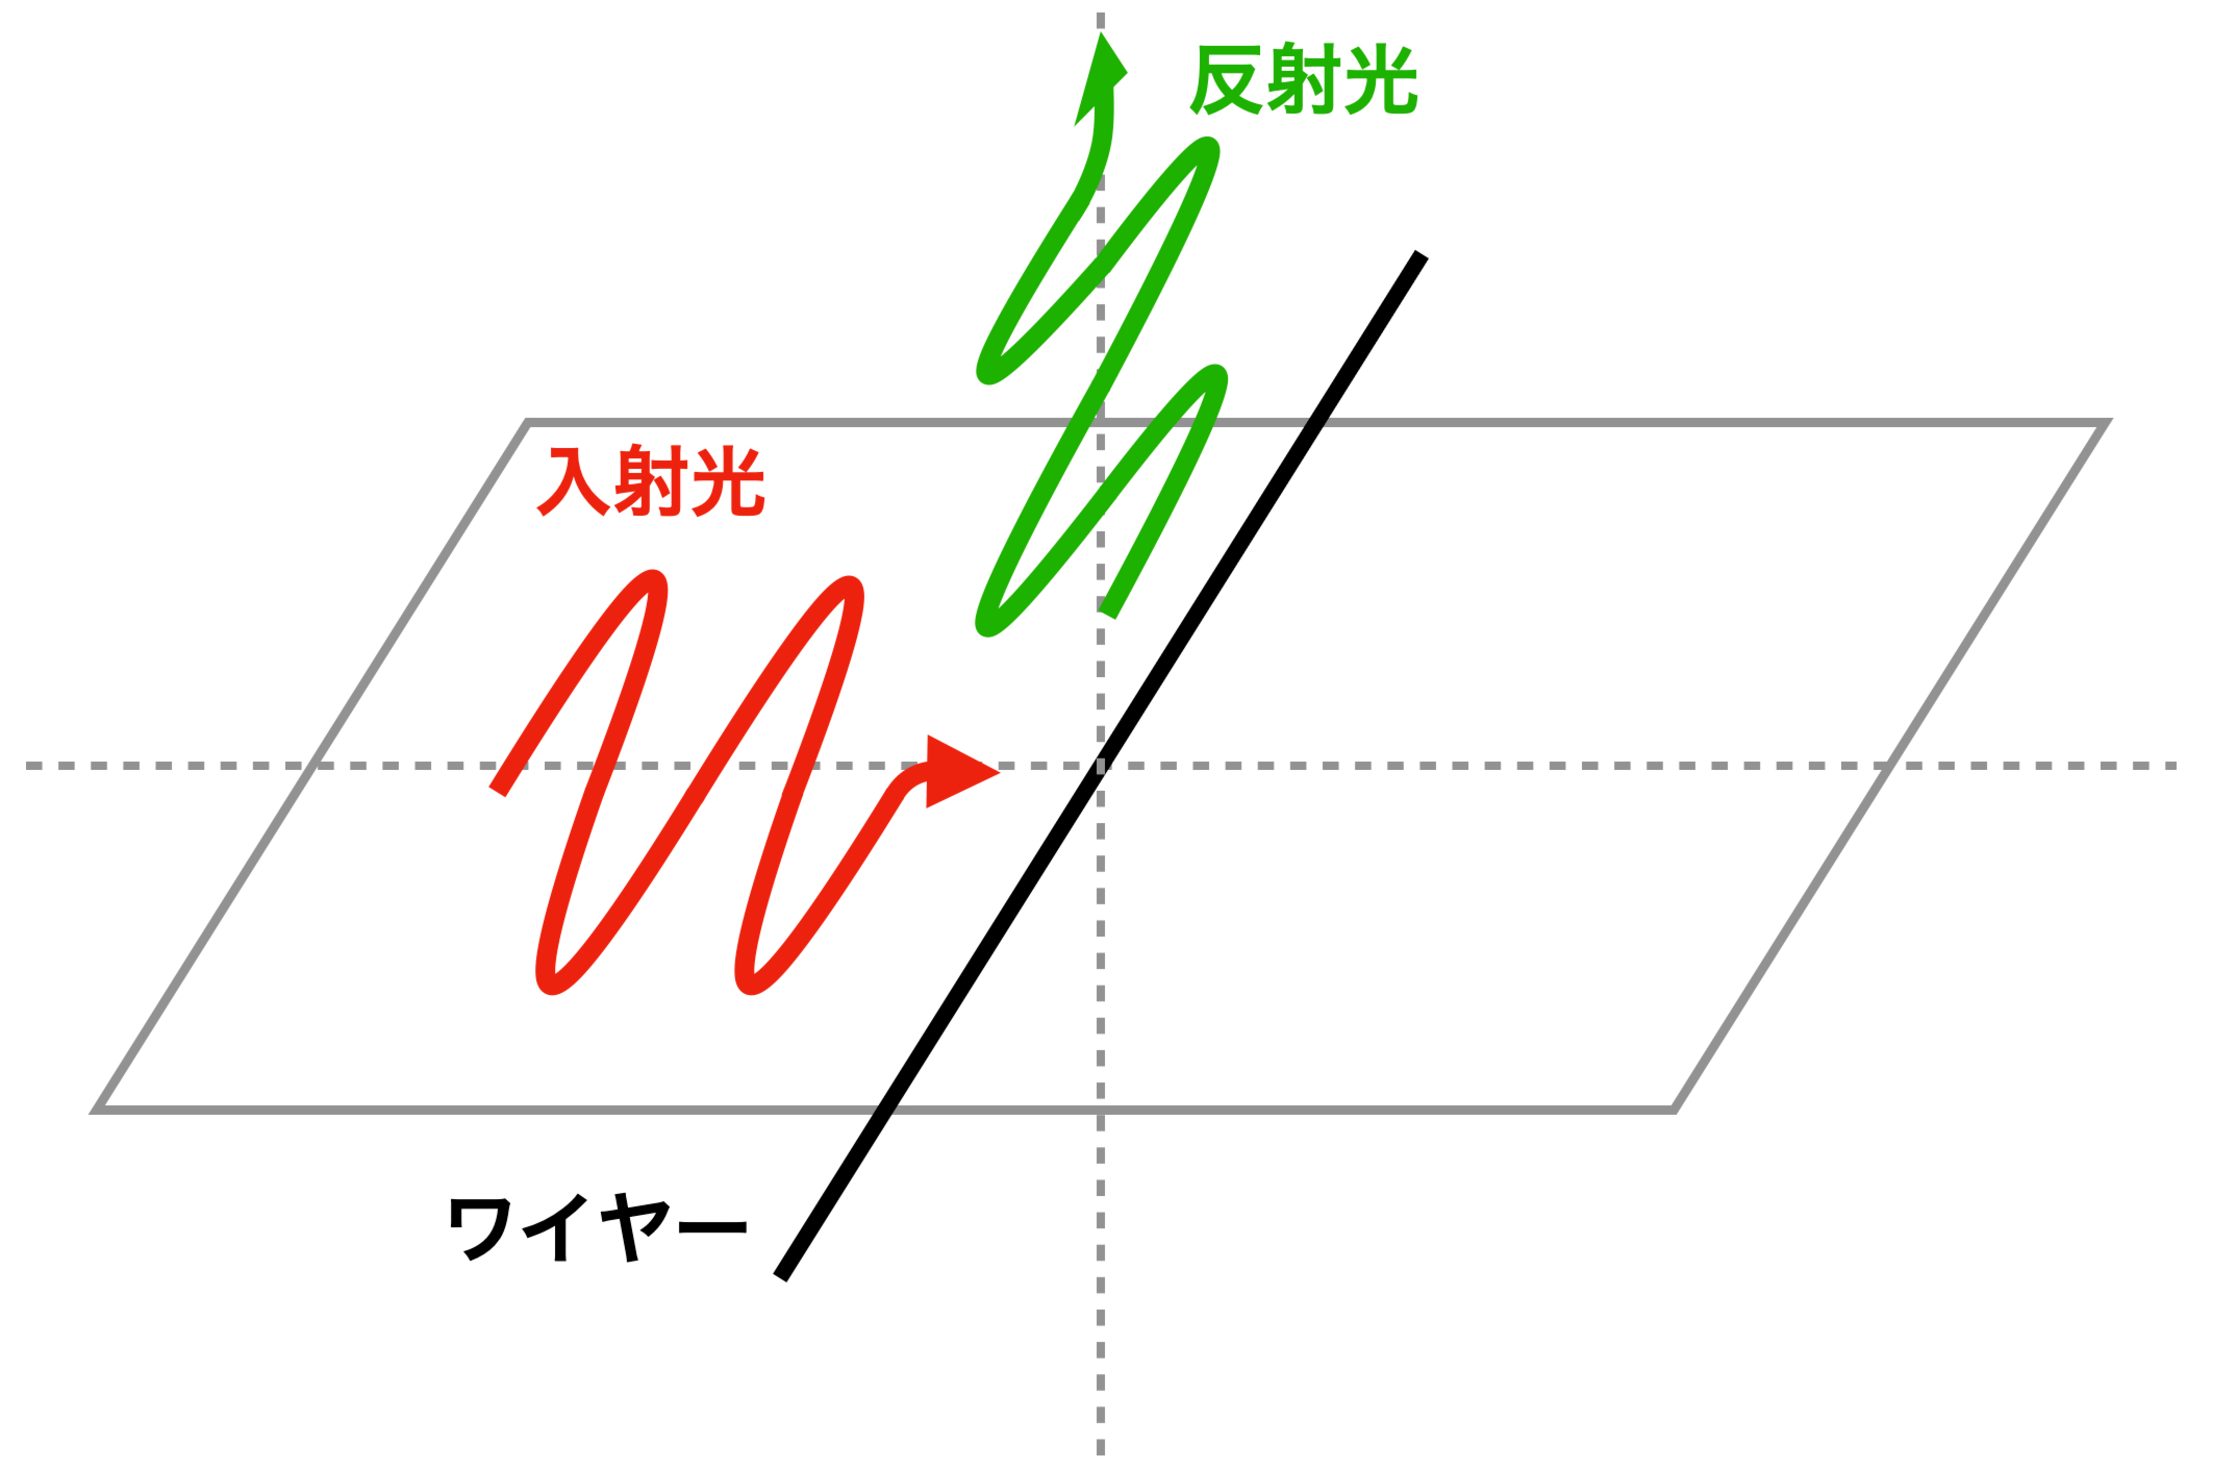
\includegraphics[width=\columnwidth]{wiregrid/wire_reflect.pdf}
        \subcaption{}
        \label{fig:wire_reflect}
    \end{minipage}
    \hspace{0.02\columnwidth}
    \begin{minipage}[b]{0.48\columnwidth}
        \centering
        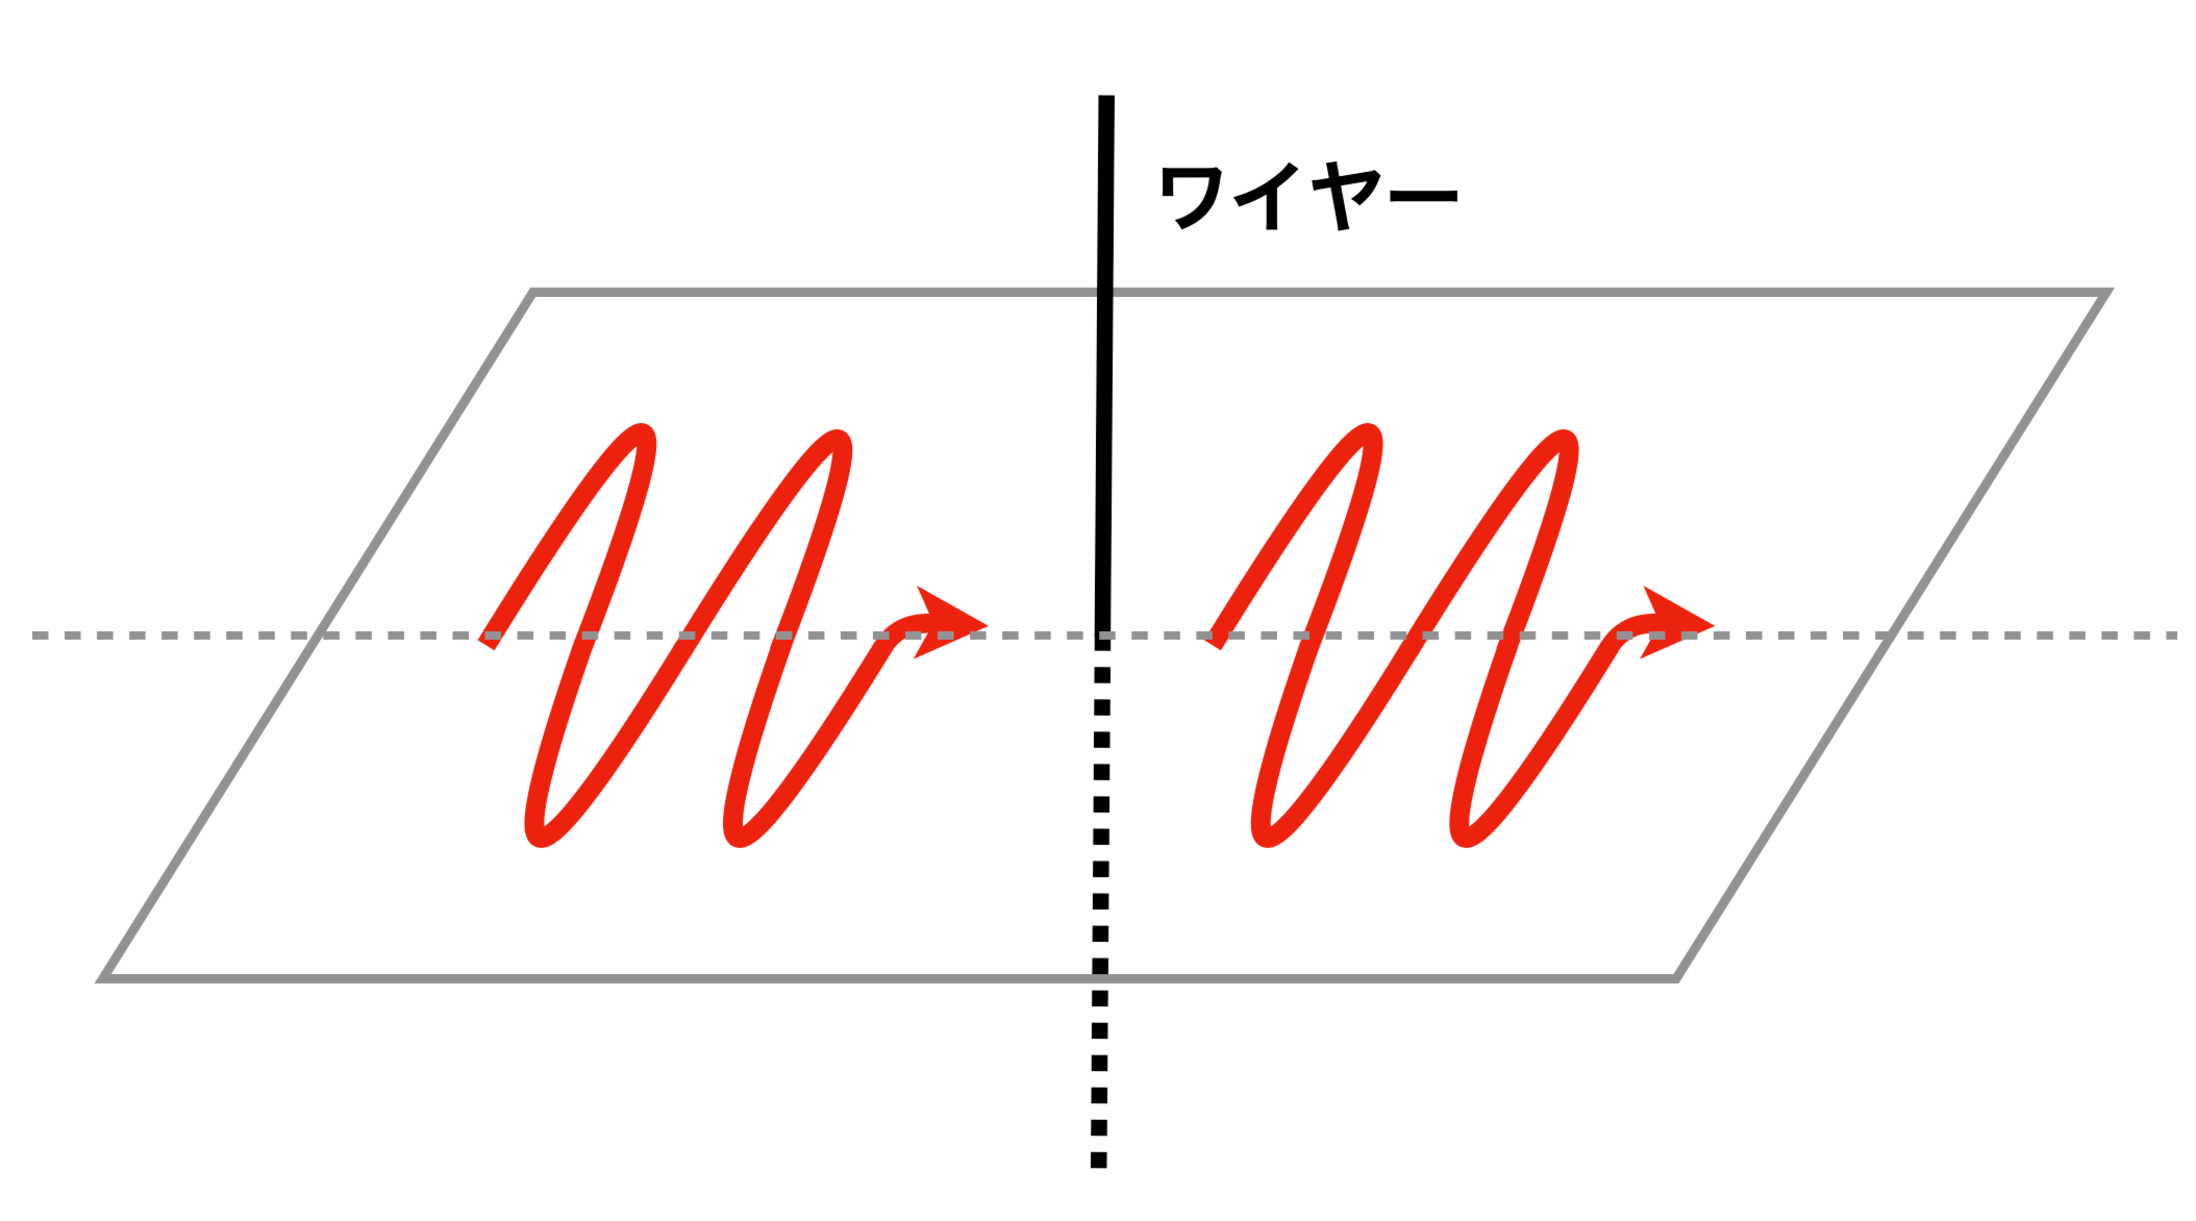
\includegraphics[width=\columnwidth]{wiregrid/wire_through.pdf}
        \subcaption{}
        \label{fig:wire_through}
    \end{minipage}
    \centering
    \caption{ワイヤーが作る偏光信号のイメージ。
             (\subref{fig:wire_reflect})はワイヤーに沿う方向に偏光した光が入射し、まわりに散乱する様子。
             (\subref{fig:wire_through})はワイヤーに対し垂直な方向に偏光した光が反射されることなく通過する様子。
             }
    \label{fig:wire_polarization}
\end{figure}
\section{偏光角較正の原理}
式\eqref{eq:so-hwp_modulation}において、入射光としてワイヤー由来の偏光角 $\theta_{\mathrm{wire}}$ の直線偏光した光を考える。
$Q_{\mathrm{in}}(t) + iU_{\mathrm{in}}(t) = \exp\qty[2i\theta_{\mathrm{wire}}]$ となるため、
\begin{equation}
    d_{\mathrm{m}, \mathrm{det}}(t) = I_{\mathrm{in}}(t) + \varepsilon\Re\qty[\exp\qty{-i \qty(4\omega_{\mathrm{HWP}}t + 4\chi_0 - 2\theta_{\mathrm{det}} - 2\theta_{\mathrm{wire}})}]
\end{equation}
となる。
ワイヤー由来の光の強度はほとんど時間変化しないため、$I_{\mathrm{in}}(t) \simeq \mathrm{const.}$ とみなせる。
したがって、この変調信号は時系列データとして位相オフセット $4\chi_0 + 2(\theta_{\mathrm{det}} + \theta_{\mathrm{wire}})$ を持った
角振動数 $4\omega_{\mathrm{HWP}}$ の正弦波としてみえる。
理想的な時系列データのイメージを図\ref{fig:}に示す。
これを復調することで、式\eqref{eq:so-hwp_demod}より
\begin{equation}
    d_{\mathrm{d, det}} = \varepsilon\exp\qty[i2\qty(\theta_{\mathrm{wire}} + \theta_{\mathrm{det}})]
    \label{eq:wiregrid_mod}
\end{equation}
という偏光情報のみを得る。
望遠鏡では光学系により生まれる偽偏光や、環境熱放射が比等方だった場合にはワイヤー角度に対して非等方な強度のワイヤー由来の偏光が観測され得る。
これを取り除くため、さまざまなワイヤーの角度 $\theta_{\mathrm{wire}}$ でこの $d_{\mathrm{d, det}}$ を測定し、複素平面上で円(較正円と呼ぶ)を描く(\ref{fig:})。
光学系による偽偏光は較正円の原点がズレる効果として現れ、環境熱放射の非等方性は較正円を歪ませる効果として現れる。
この較正円を用いて補正を加え、最終的に検出器の偏光角 $\theta_{\mathrm{det}}$ を較正する。
\begin{figure}[tbp]
    \centering
    % \includegraphics[draft, width=0.5]{wiregrid/hogehoge.pdf}
    \caption[スパースワイヤーグリッドによって生成される偏光信号の時系列データイメージ]{スパースワイヤーグリッドによって生成される偏光信号の時系列データイメージ}
\end{figure}
\begin{figure}[tbp]
    \centering
    % \includegraphics[draft, width=0.5]{wiregrid/hogehoge.pdf}
    \caption{較正円のイメージ}
\end{figure}
\section{較正装置の設計と特徴}
較正円を描くためにはスパースワイヤーグリッドを回転させ、ワイヤーの角度を変化させる必要がある。
また、本装置は望遠鏡の窓の前に設置されるという特性上、CMB観測時にはそれを取り外さなければならない。
先行研究ではこのような回転・切り替え作業を手動にて行ってきたが、それに伴って短期間での再較正が困難であった。
そこで、本装置ではワイヤーの回転と観測・較正の切り替えを自動で行う機構が開発・搭載され、10分程度での較正が実現されている。
本節では、スパースワイヤーグリッド本体の設計に加え、この自動化機構について述べる。
\subsection{スパースワイヤーグリッドの設計}
スパースワイヤーグリッドの概観を図\ref{fig:swg}(\subref{fig:wiregrid_appearance})に示す。
これは金属製のワイヤーを、入射光よりも十分長い間隔で平行に張ったものであり、ワイヤー軸に沿った偏光を生成する。
SOではアルミニウム製の内径$\SI{790}{mm}$、外径 $\SI{830}{mm}$ の円環に、直径 $\SI{0.1}{mm}$ の
タングステンワイヤーを $\SI{20}{mm}$ 間隔で $39$ 本張り巡らせたものを使用する\cite{swg:murata}。

アルミニウムリング上には $\SI{0.2}{mm}$ の幅で刻まれた溝があり、これによりワイヤーの位置を決める。
$\SI{230}{g}$ の重りをワイヤーにくくりつけることでピンと張った状態にし、この溝の上にワイヤーが沿うように設置したのち、
Henkel 社製 の LOCTITE STYCAST 2850FTJ という接着剤を用いて固定する。
接着剤による固定部分はサンドブラストされたネジ頭となっており、このネジを取り替えることで接着後であってもワイヤーを張り直すことができるようになっている。
図\ref{fig:swg}(\subref{fig:wire_detail_view})にワイヤー接着部分の詳細を示す。
\begin{figure}[H]
    \begin{minipage}[b]{0.48\columnwidth}
        \centering
        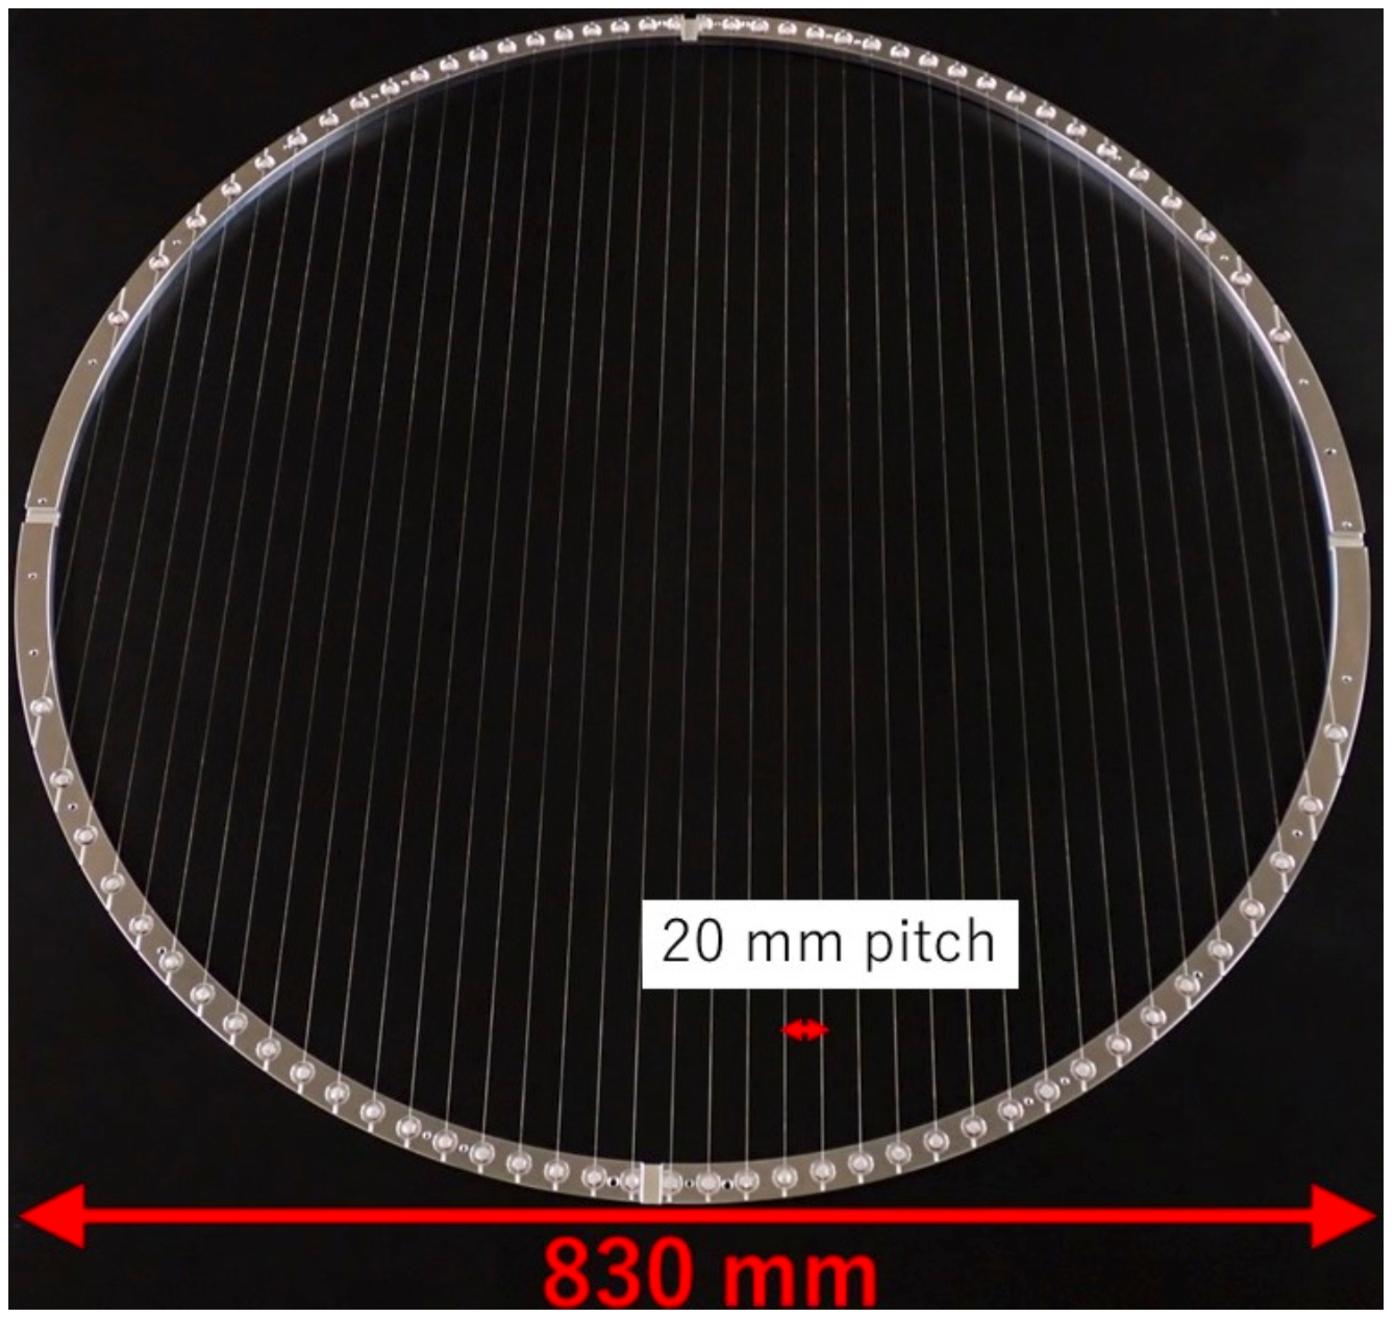
\includegraphics[width=\columnwidth]{wiregrid/wiregrid_appearance.pdf}
        \subcaption{}
        \label{fig:wiregrid_appearance}
    \end{minipage}
    \hspace{0.02\columnwidth}
    \begin{minipage}[b]{0.48\columnwidth}
        \centering
        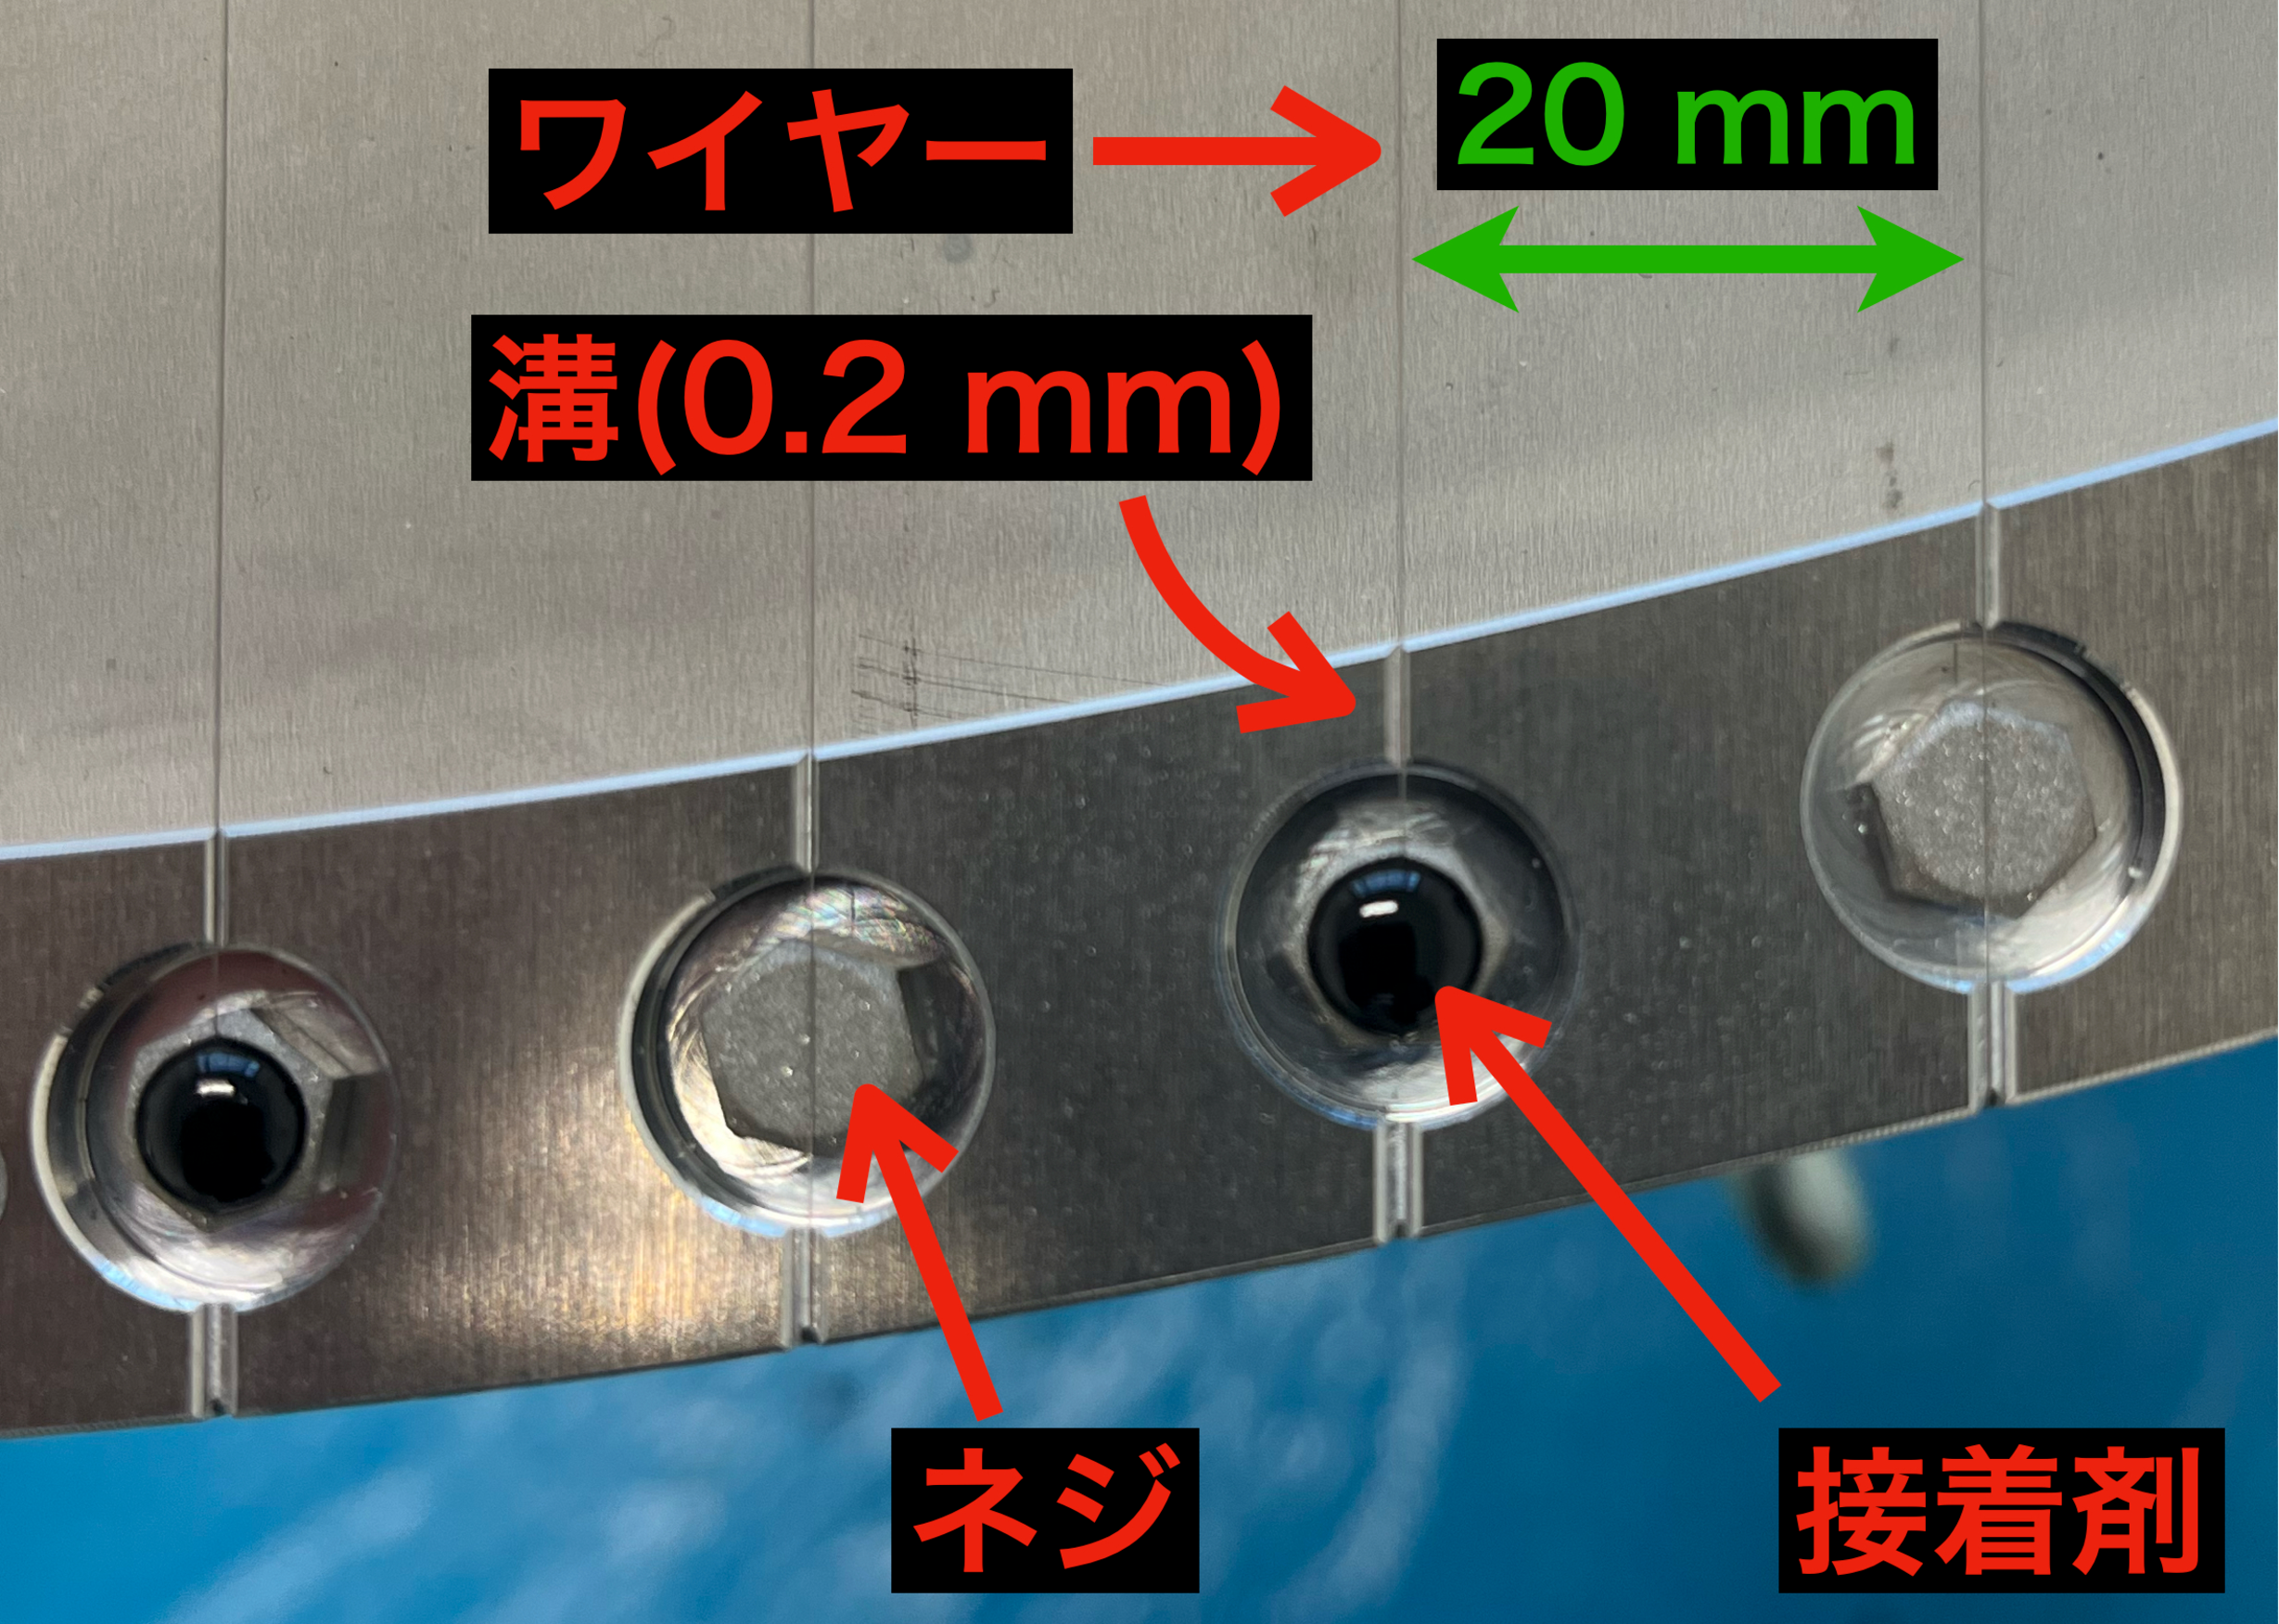
\includegraphics[width=\columnwidth]{wiregrid/wire_detail_view.pdf}
        \subcaption{}
        \label{fig:wire_detail_view}
    \end{minipage}
    \caption{(\subref{fig:wiregrid_appearance})スパースワイヤーグリッドの概観~\cite{swg:Murata_2023}\ (\subref{fig:wire_detail_view})ワイヤー接着部分の詳細}
    \label{fig:swg}
\end{figure}
\begin{figure}[H]
    \centering
    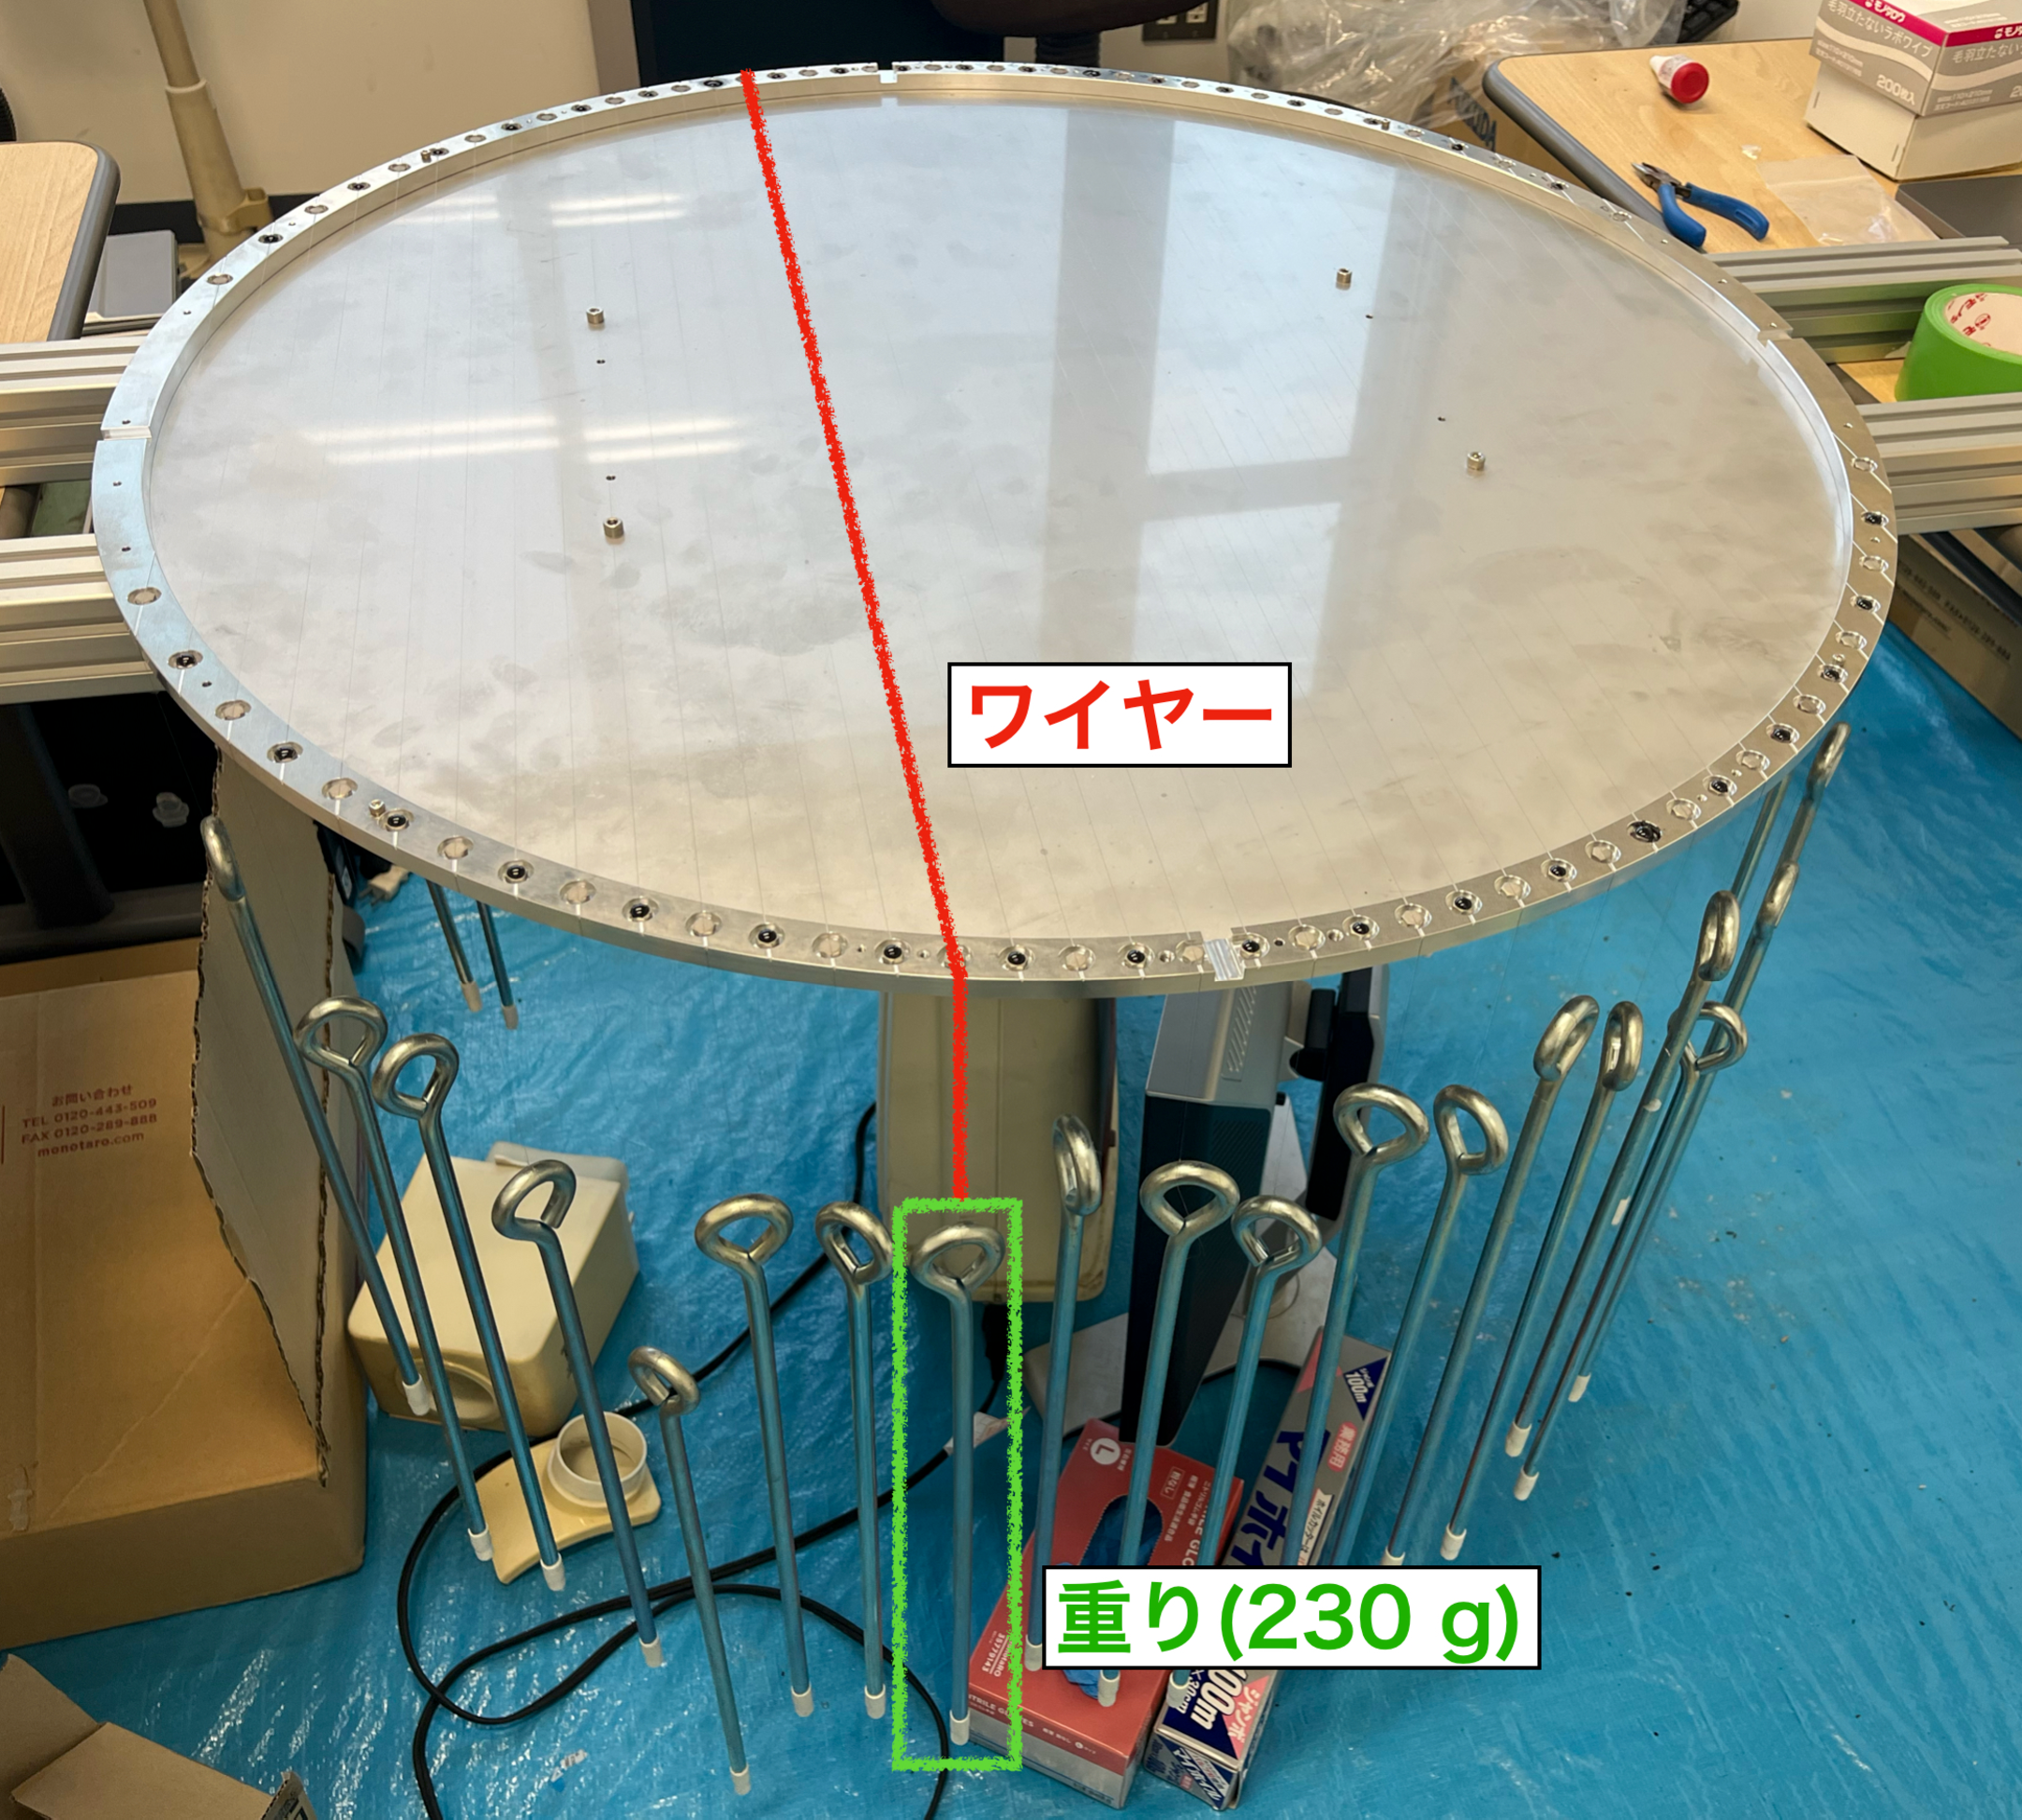
\includegraphics[width=0.8\textwidth]{wiregrid/wire_attachment.pdf}
    \caption[ワイヤーを張るときの様子]{ワイヤーを張るときの様子。ワイヤーの両端に $\SI{230}{g}$ の重りをつけ、張力をかけている。}
    \label{fig:wire_attachment}
\end{figure}
\subsection{回転機構}
Crouzet USA 社製の STANDARD MOTOR 2900 RPM 12V というDCモーターを使用し、スパースワイヤーグリッドを回転させる。
図\ref{fig:rotation_parts}に回転機構の概観を示す。
回転角度は RENISHAW 社製の LM15IC という角度にして $0.004\tcdegree$ の分解能を持つ磁気エンコーダを用いて測定されており、$0.03\tcdegree$ の精度で常にモニターされる。
モニターされた角度を用いてDCモーターへの電流を制御するシステムが開発されており、
これによりスパースワイヤーグリッドを$\order{1\tcdegree}$ の精度で $22.5\tcdegree$ ずつ回転させ、較正円を描く\cite{swg:nakata}。
\subsection{切り替え機構}
本較正装置ではCMB観測モードと較正モードの切り替えを2本のアクチュエータによって
スパースワイヤーグリッドを出し入れすることで実現している。
図\ref{fig:gridloader}に切り替え機構の概観を示す。
アクチュエータのモーターには Oriental motor 社製の PK269JDA という2相式ステッピングモーターを使用しており、
アクチュエータの両端にあるリミットスイッチによりスパースワイヤーグリッドが端まで移動したことを認識、動作を止める。
本機構によるスパースワイヤーグリッドの出し入れは片道で $90$ 秒程度となっており、CMB観測の時間を無駄にすることなく較正を行うことに貢献している\cite{swg:nakata}。
\begin{figure}[H]
    \centering
    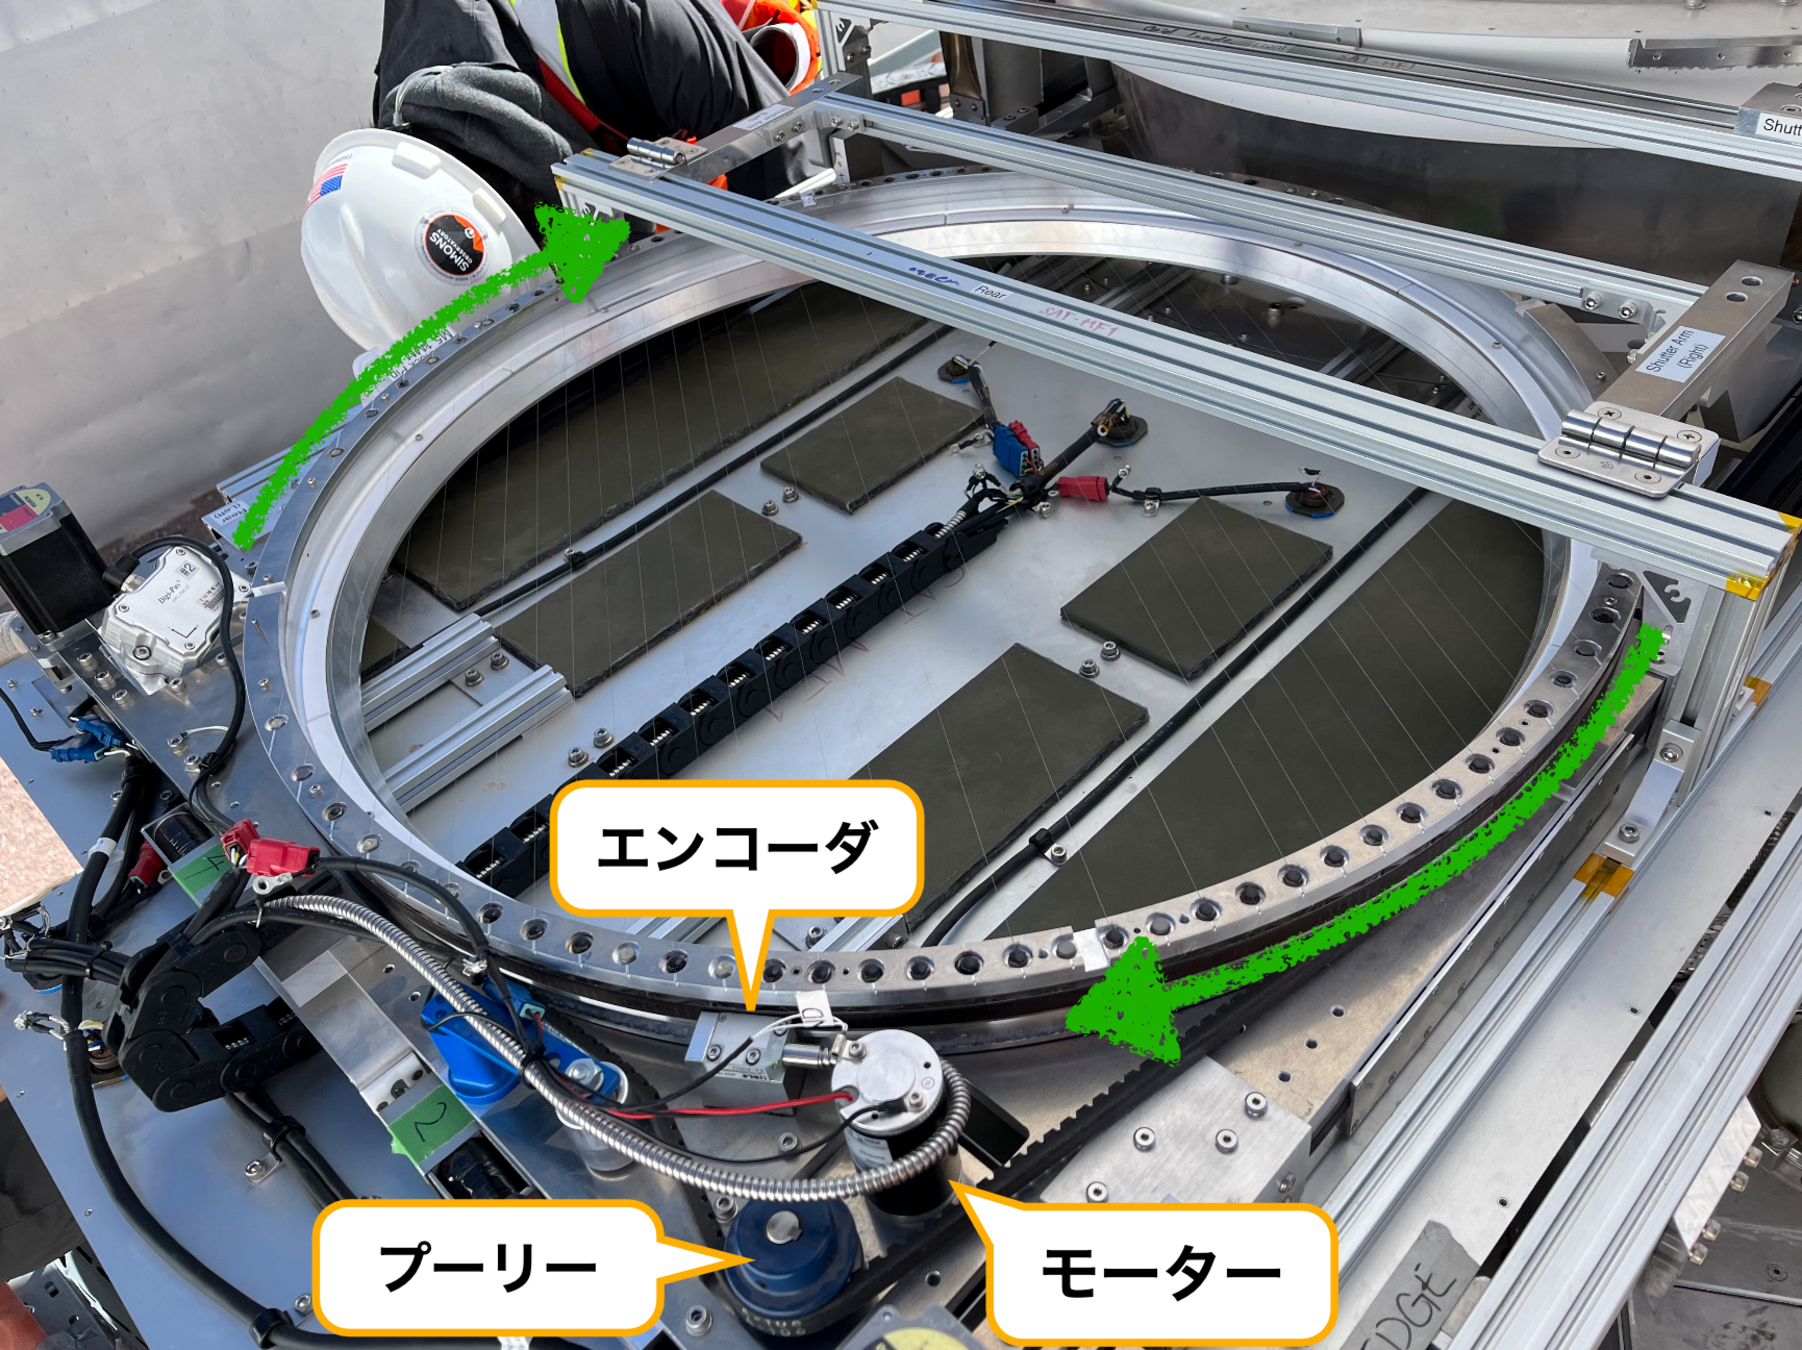
\includegraphics[width=0.65\textwidth]{wiregrid/rotation_parts.pdf}
    \caption{スパースワイヤーグリッドに搭載された回転機構の概観}
    \label{fig:rotation_parts}
\end{figure}
\begin{figure}[H]
    \centering
    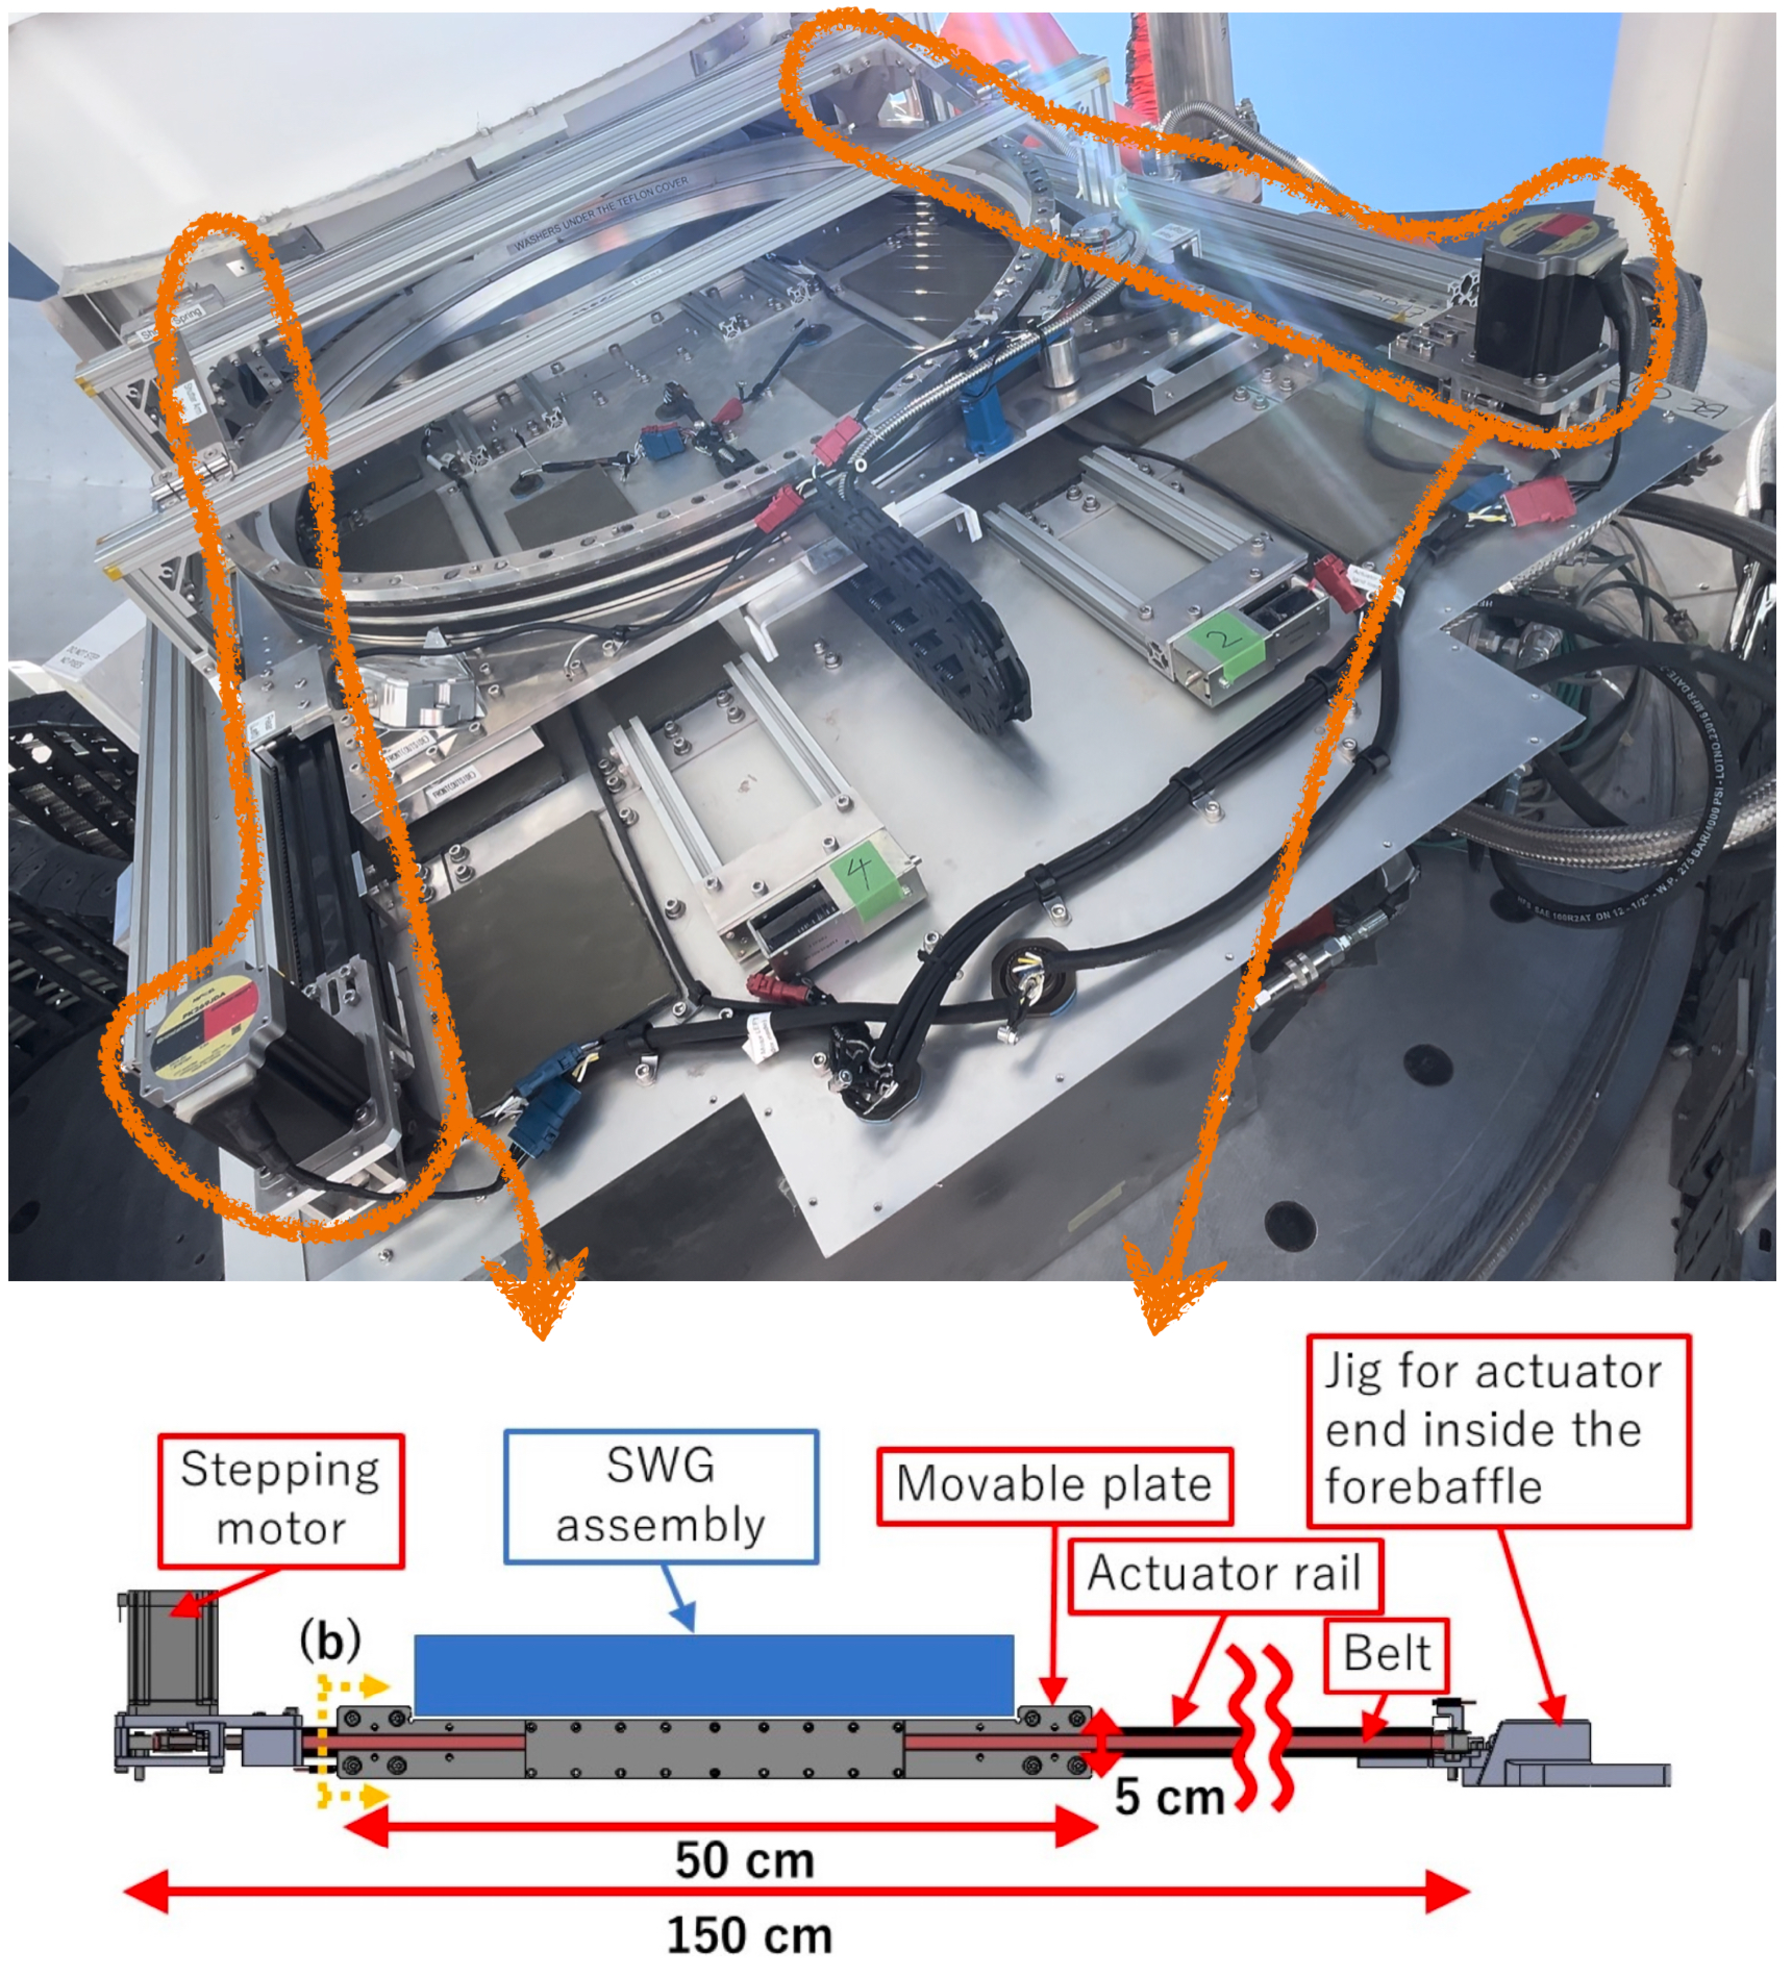
\includegraphics[width=0.65\textwidth]{wiregrid/wiregrid_actuator.pdf}
    \caption[スパースワイヤーグリッドに搭載された切り替え機構の概観]{スパースワイヤーグリッドに搭載された切り替え機構の概観。
    上図が観測サイトにインストールされた較正装置であり、オレンジの線で囲んだ部分の詳細を下図に示している。
    \colortext{blue}{初見で分かりにくい?もう少しまともな図を作りたい。}
    }
    \label{fig:gridloader}
\end{figure}
\subsection{重力参照計}
\subsubsection{重力参照計を用いた $\theta_{\mathrm{wire}}$ の測定}
式\eqref{eq:wiregrid_mod}において、 $\theta_{\mathrm{wire}}$ は天球面上におけるワイヤーが作り出す偏光角(絶対角度)である。
エンコーダはスパースワイヤーグリッドがその平面内において回転したワイヤーの角度(相対角度)を出力するので、
別の手段を用いてこの平面が天球面上のどこに位置しているかを知る必要がある。
これを知るために、重力を参照してその平面がどう傾いているのかを出力する2軸の重力参照計を導入する。
ここでは、絶対角度がどのように測られるかについて述べる。

図\ref{fig:abs_angle}(\subref{fig:abs_angle_overview})のように各種平面、角度を定義する。$xy$ 平面として重力に対して垂直な平面を取り、$z$ 軸負の方向が重力方向となるように座標系を取る。
図中に円環として描かれているのがスパースワイヤーグリッドであり、重力参照計が持つ2軸を $x',\,y'$ 軸とする。
$\alpha,\,\beta$ は重力参照計が測定する角度であり、$x',\,y'$ 軸が $xy$ 平面となす角度である。
図中にある horizontal line とは、$xy$ 平面と $x',\,y'$ 平面が交わる直線である。
以上の定義から、$x'$ 軸と horizontal line がなす角 $\theta_{\mathrm{sens}}$ は
\begin{equation}
    \theta_{\mathrm{sens}} = \arctan\qty(\dfrac{\sin\alpha}{\sin\beta})
\end{equation}
と表される\cite{swg:Murata_2023}。
図\ref{fig:abs_angle}(\subref{fig:abs_angle_WG_plane})にスパースワイヤーグリッド平面における各種測定角度と、
ワイヤーの絶対角度 $\theta_{\mathrm{wire}}$ の関係を示す。
$\theta_{\mathrm{enc}}$ はエンコーダによって測定された値であり、$\theta_{\mathrm{enc}0}$ はエンコーダの零点と $x'$ 軸のなす角である。
以上を用いることで、絶対角度は
\begin{equation}
    \theta_{\mathrm{wire}} = \theta_{\mathrm{enc}} + \theta_{\mathrm{enc}0} + \theta_{\mathrm{sens}}
\end{equation}
と測定される。
\begin{figure}[tbp]
    \begin{minipage}[b]{0.48\columnwidth}
        \centering
        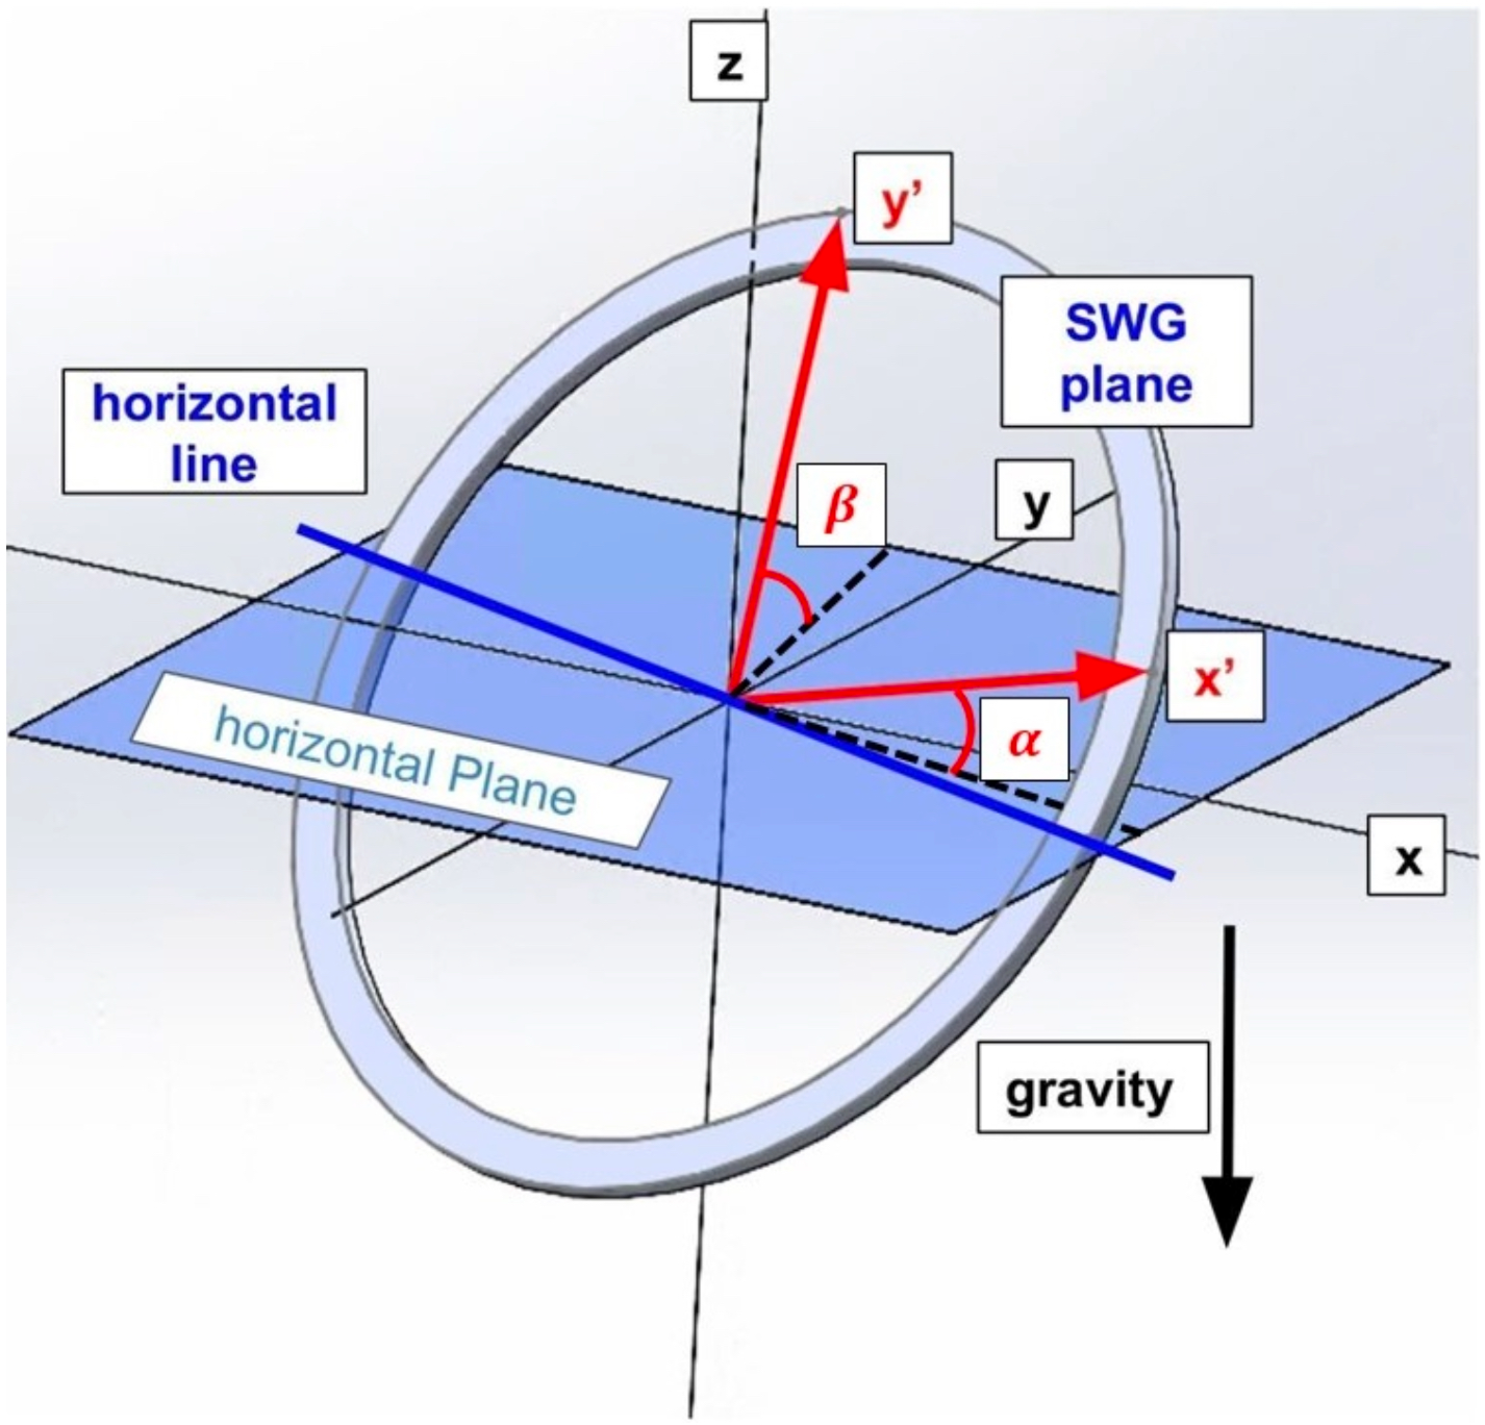
\includegraphics[width=\columnwidth]{wiregrid/abs_angle_overview.pdf}
        \subcaption{}
        \label{fig:abs_angle_overview}
    \end{minipage}
    \hspace{0.06\columnwidth}
    \begin{minipage}[b]{0.40\columnwidth}
        \centering
        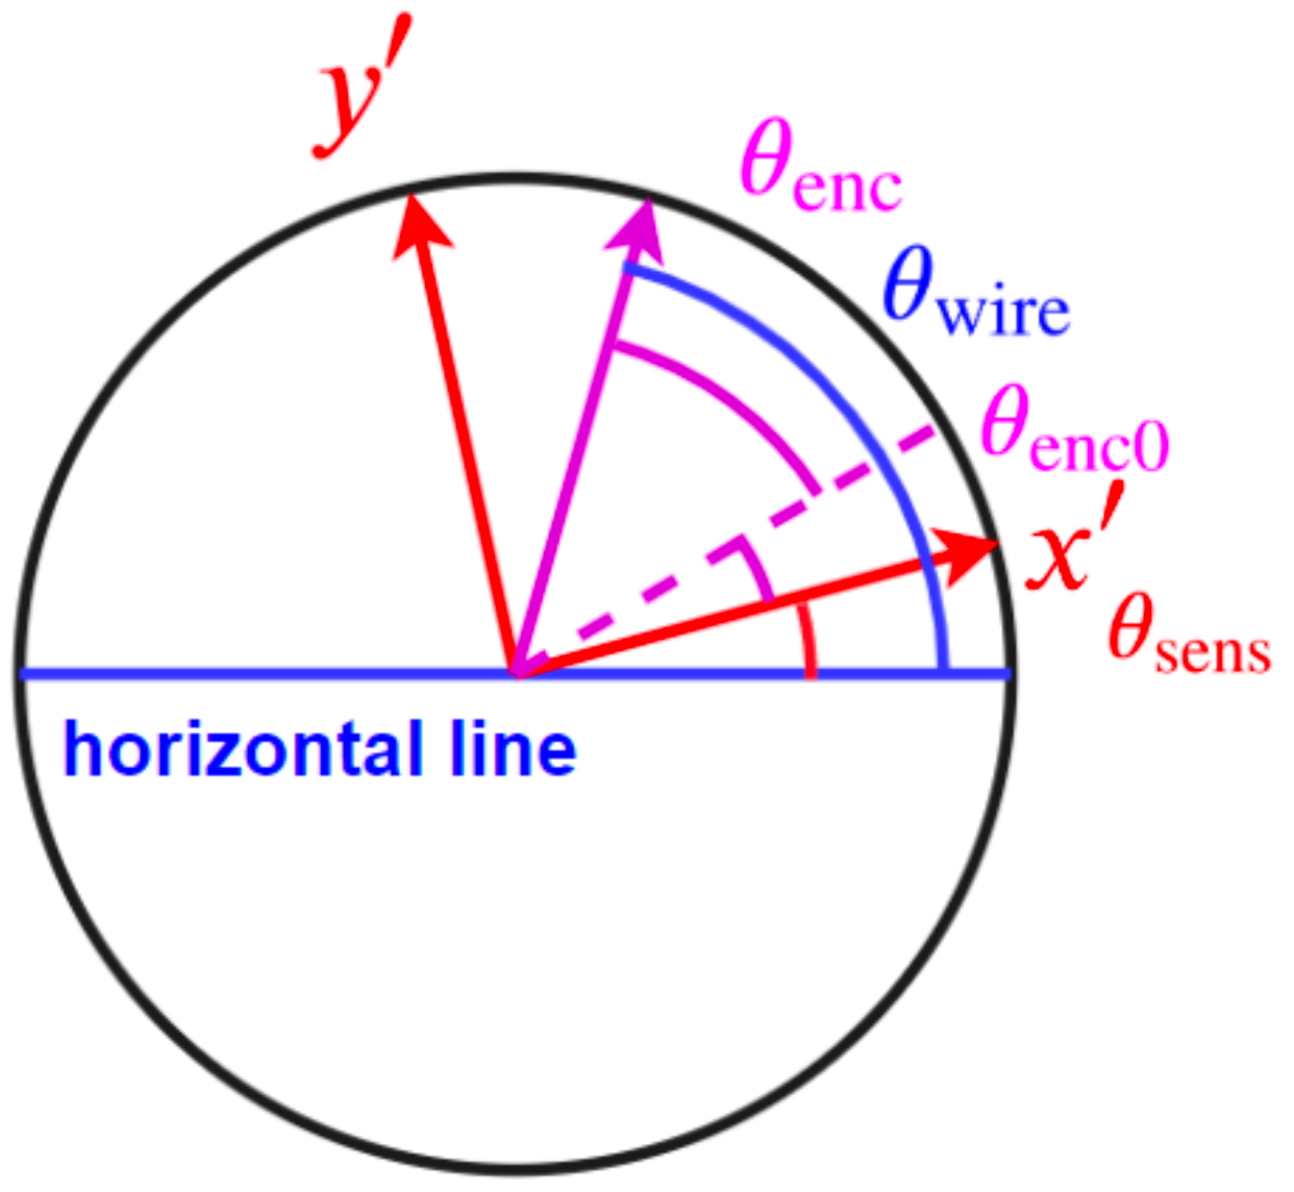
\includegraphics[width=\columnwidth]{wiregrid/abs_angle_WG_plane.pdf}
        \subcaption{}
        \label{fig:abs_angle_WG_plane}
    \end{minipage}
    \caption{(\subref{fig:abs_angle_overview})絶対角度測定のための各種平面と角度の定義 (\subref{fig:abs_angle_WG_plane})スパースワイヤーグリッド平面における回転角と絶対角度}
    \label{fig:abs_angle}
\end{figure}

\subsubsection{重力参照計の設置}
図\ref{fig:tiltsensor_at_site}に重力参照計の設置状況を示す。
重力参照計はスパースワイヤーグリッドの回転機構のベースプレートに取り付けられている。
SATはelevation $50\tcdegree$ での観測を主要としており、
スパースワイヤーグリッドは boresight $60\tcdegree$ のオフセットを持って設置されているため、
これらのオフセットを打ち消し、重力参照計が両軸ともに $0\tcdegree$ を指すように設置されている。
また、重力参照計は自身のX軸、Y軸が重力に対して


\begin{figure}[H]
    \centering
    \includegraphics[width=0.8\textwidth]{wiregrid/tiltsensor_at_site.pdf}
    \caption{重力参照計の設置状況}
    \label{fig:tiltsensor_at_site}
\end{figure}

\section{系統誤差}
本節では、ワイヤーの絶対角度を測定するにあたって考えられる系統誤差の要因と、先行研究によって評価されたその値について述べる。
その後、評価を見直すべき点をまとめ、本論文の位置付けについて述べる。
\subsection{ワイヤーの設置精度に伴う系統誤差}
ワイヤーは $\SI{0.2}{mm}$ の溝に沿うような形で設置される。
この範囲でのみワイヤーは動くと考えると、アルミニウムリングの中心部では $0.02\tcdegree$ の精度でワイヤーを張ることが可能である。
この系統誤差は機械工作精度によって決まっている。
\subsection{エンコーダの測定精度に伴う系統誤差}
\ref{}にて述べた磁気エンコーダが行う回転角度 $\theta_{\mathrm{enc}}$ の測定において、
磁気エンコーダ自体の角度分解能は $0.004\tcdegree$ に相当する。
しかし、回転機構のベアリングのステーターと巻きつけられた磁気テープの中心が完全に一致しない偏心の影響や、
磁気テープが巻き付けられる回転部分の金属部品が工作精度の下で楕円に歪むことの影響を受け、
$\theta_{\mathrm{enc}}$ の精度は必ずしも $0.004\tcdegree$ になるとは限らない。
先行研究~\cite{swg:iijima}では Faro 社製の3次元測定器 Faro Edge を用いてこの精度を確認し、
その精度として $0.03\tcdegree$ を得ている。
\subsection{エンコーダの零点測定に伴う系統誤差}
$\theta_{\mathrm{enc}0}$ は実験室にて測られるエンコーダの零点である。
ワイヤーの絶対角度が $\theta_{\mathrm{wire}} = 0\tcdegree$ となった状態で $\theta_{\mathrm{enc}}$ と $\theta_{\mathrm{sens}}$ を測定することで決定され、
その精度は $0.04\tcdegree$ と測定されている~\cite{swg:iijima}。\\
\colortext{blue}{もう少し測定方法について述べるべきだろうか?}

\subsection{重力参照計の精度に伴う系統誤差}
重力参照計が出力する角度の精度は、$\theta_{\mathrm{sens}}$ の誤差として現れる。
これまで、Digi-Pas 社製の DWL5000-XY という製品の使用を予定されていたが、先行研究\cite{swg:iijima}にてその精度を欠き、
SOにおける要求絶対角度較正精度 $\delta\theta \leq 0.1\tcdegree$ を満たさないことが示された。

\subsection{ワイヤーのたわみに伴う系統誤差}
較正に使う光はワイヤーに沿う形で生成されるため、ワイヤーがたわんでいる部分から生成される光はその偏光角が
ワイヤーの絶対角度 $\theta_{\mathrm{wire}}$ からずれてしまい、系統誤差になる。
本項では、先行研究\cite{swg:murata}および\cite{swg:iijima}にて行われているワイヤーのたわみ量の評価について述べる。

\begin{figure}[H]
    \centering
    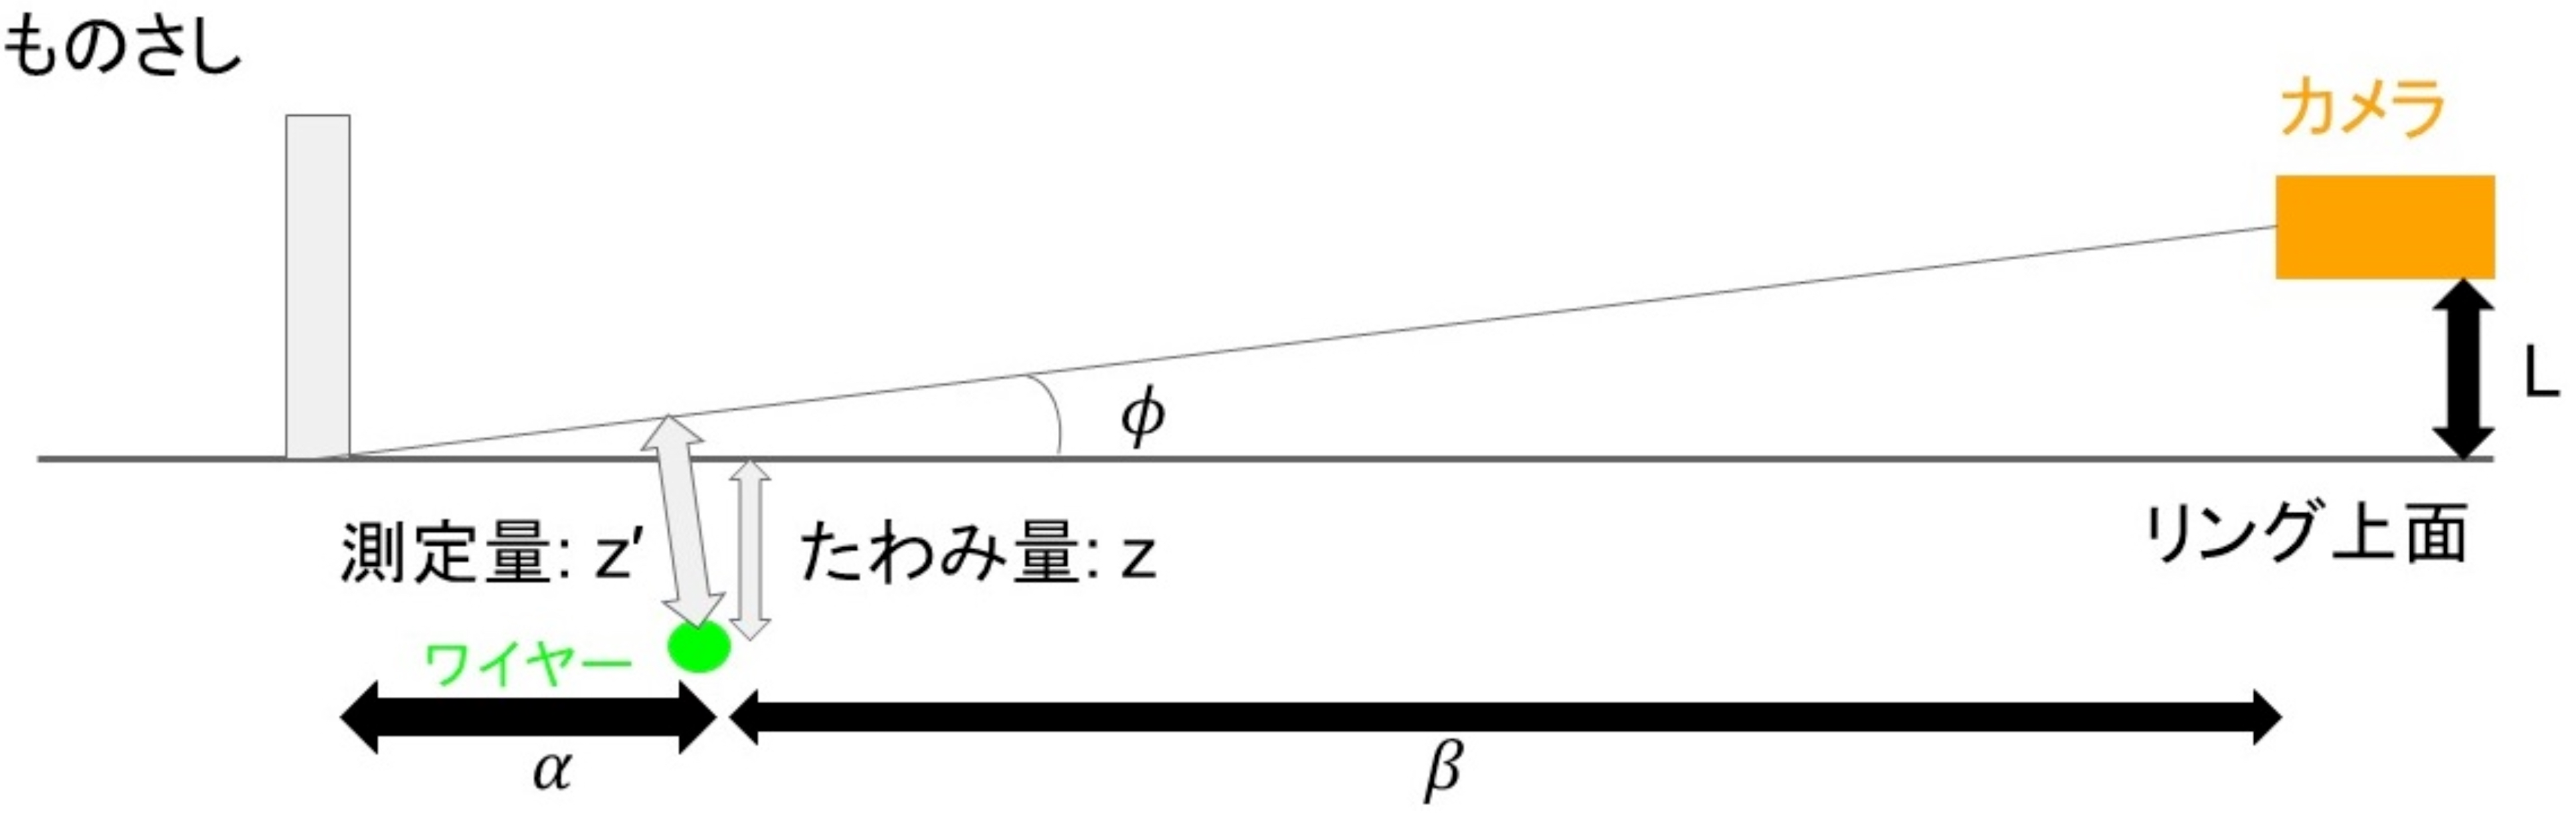
\includegraphics[width=0.8\textwidth]{wiregrid/wiresag_setup_old.pdf}
    \caption{先行研究におけるワイヤーのたわみ量評価系のセットアップ\cite{swg:murata}}
    \label{fig:wiresag_setup_old}
\end{figure}
\begin{table}[H]
    \centering
    \caption{たわみ量評価における各種パラメータの定義}
    \begin{tabular}{|c|c|}
        \hline
        パラメータ & 定義 \\
        \hline
        $L$ & アルミニウムリング上面からカメラまでの鉛直距離 \\
        $\phi$ & ストレートエッジの下端を見るカメラの視線がリング上面となす角 \\
        $\alpha$ & ストレートエッジからワイヤーまでの水平距離 \\
        $\beta$ & カメラからワイヤーまでの水平距離 \\
        $z_{\mathrm{s}}$ & ストレートエッジの真直度 \\
        $z$ & ワイヤーのたわみ量 \\
        $z'$ & カメラで撮影した画像から測定されるストレートエッジとワイヤーの距離 \\
        \hline
    \end{tabular}
    \label{tab:wiresag_setup_old}
\end{table}
スパースワイヤーグリッドを重力に対して垂直な水平面上に置き、その上に十分な真直度が保証されたストレートエッジを置く。
ストレートエッジの位置をワイヤーの近くに調節し、横からカメラで撮影すると、撮影された画像におけるストレートエッジとワイヤーの間の距離 $z'$ を測定できる。
セットアップの概念図を図\ref{fig:wiresag_setup_old}に示す。
使用されたストレートエッジは大西測定株式会社製の 140-1000B であり、このストレートエッジは真直度A級 $\SI{30}{\mu m}$ が保証されている。
各種パラメータを表\ref{tab:wiresag_setup_old}のように定義すると、$z'$ と実際のワイヤーのたわみ $z$ の間の関係は
\begin{align}
    z &= \dfrac{z'}{\cos\phi} - \alpha\tan\phi - z_{\mathrm{s}} \\
    \phi &= \arctan\qty(\dfrac{L}{\alpha+\beta})
\end{align}
となる。

写真はワイヤーの中央と両端の3箇所で撮影された。
両端で測定される $z$ はたわみのオフセットであり、中央で測定された $z$ からこのオフセットを差し引いたものが正味のたわみ量として測定された。
また、ストレートエッジにはスケーラを貼り付けており、スケーラの目盛が写真のpixel数にしていくつなのかを測ることで
$\SI{1}{pixel}$ が何\,$\mathrm{mm}$ に対応するのか較正している。

実際に撮影された写真を図\ref{fig:wiresag_picture_old}に示す。
撮影された写真に対して、先行研究\cite{swg:murata}では画像寸法測定ツール「Click Measure」を用いて手動で、
\cite{swg:iijima}ではOpenCVライブラリを用いて二値化して、検出したストレートエッジの端とワイヤーの中心位置の距離を算出し、
ワイヤーのたわみ量を $\theta_{\mathrm{sag}} < 0.05\tcdegree$ と評価している。

\begin{figure}[H]
    \centering
    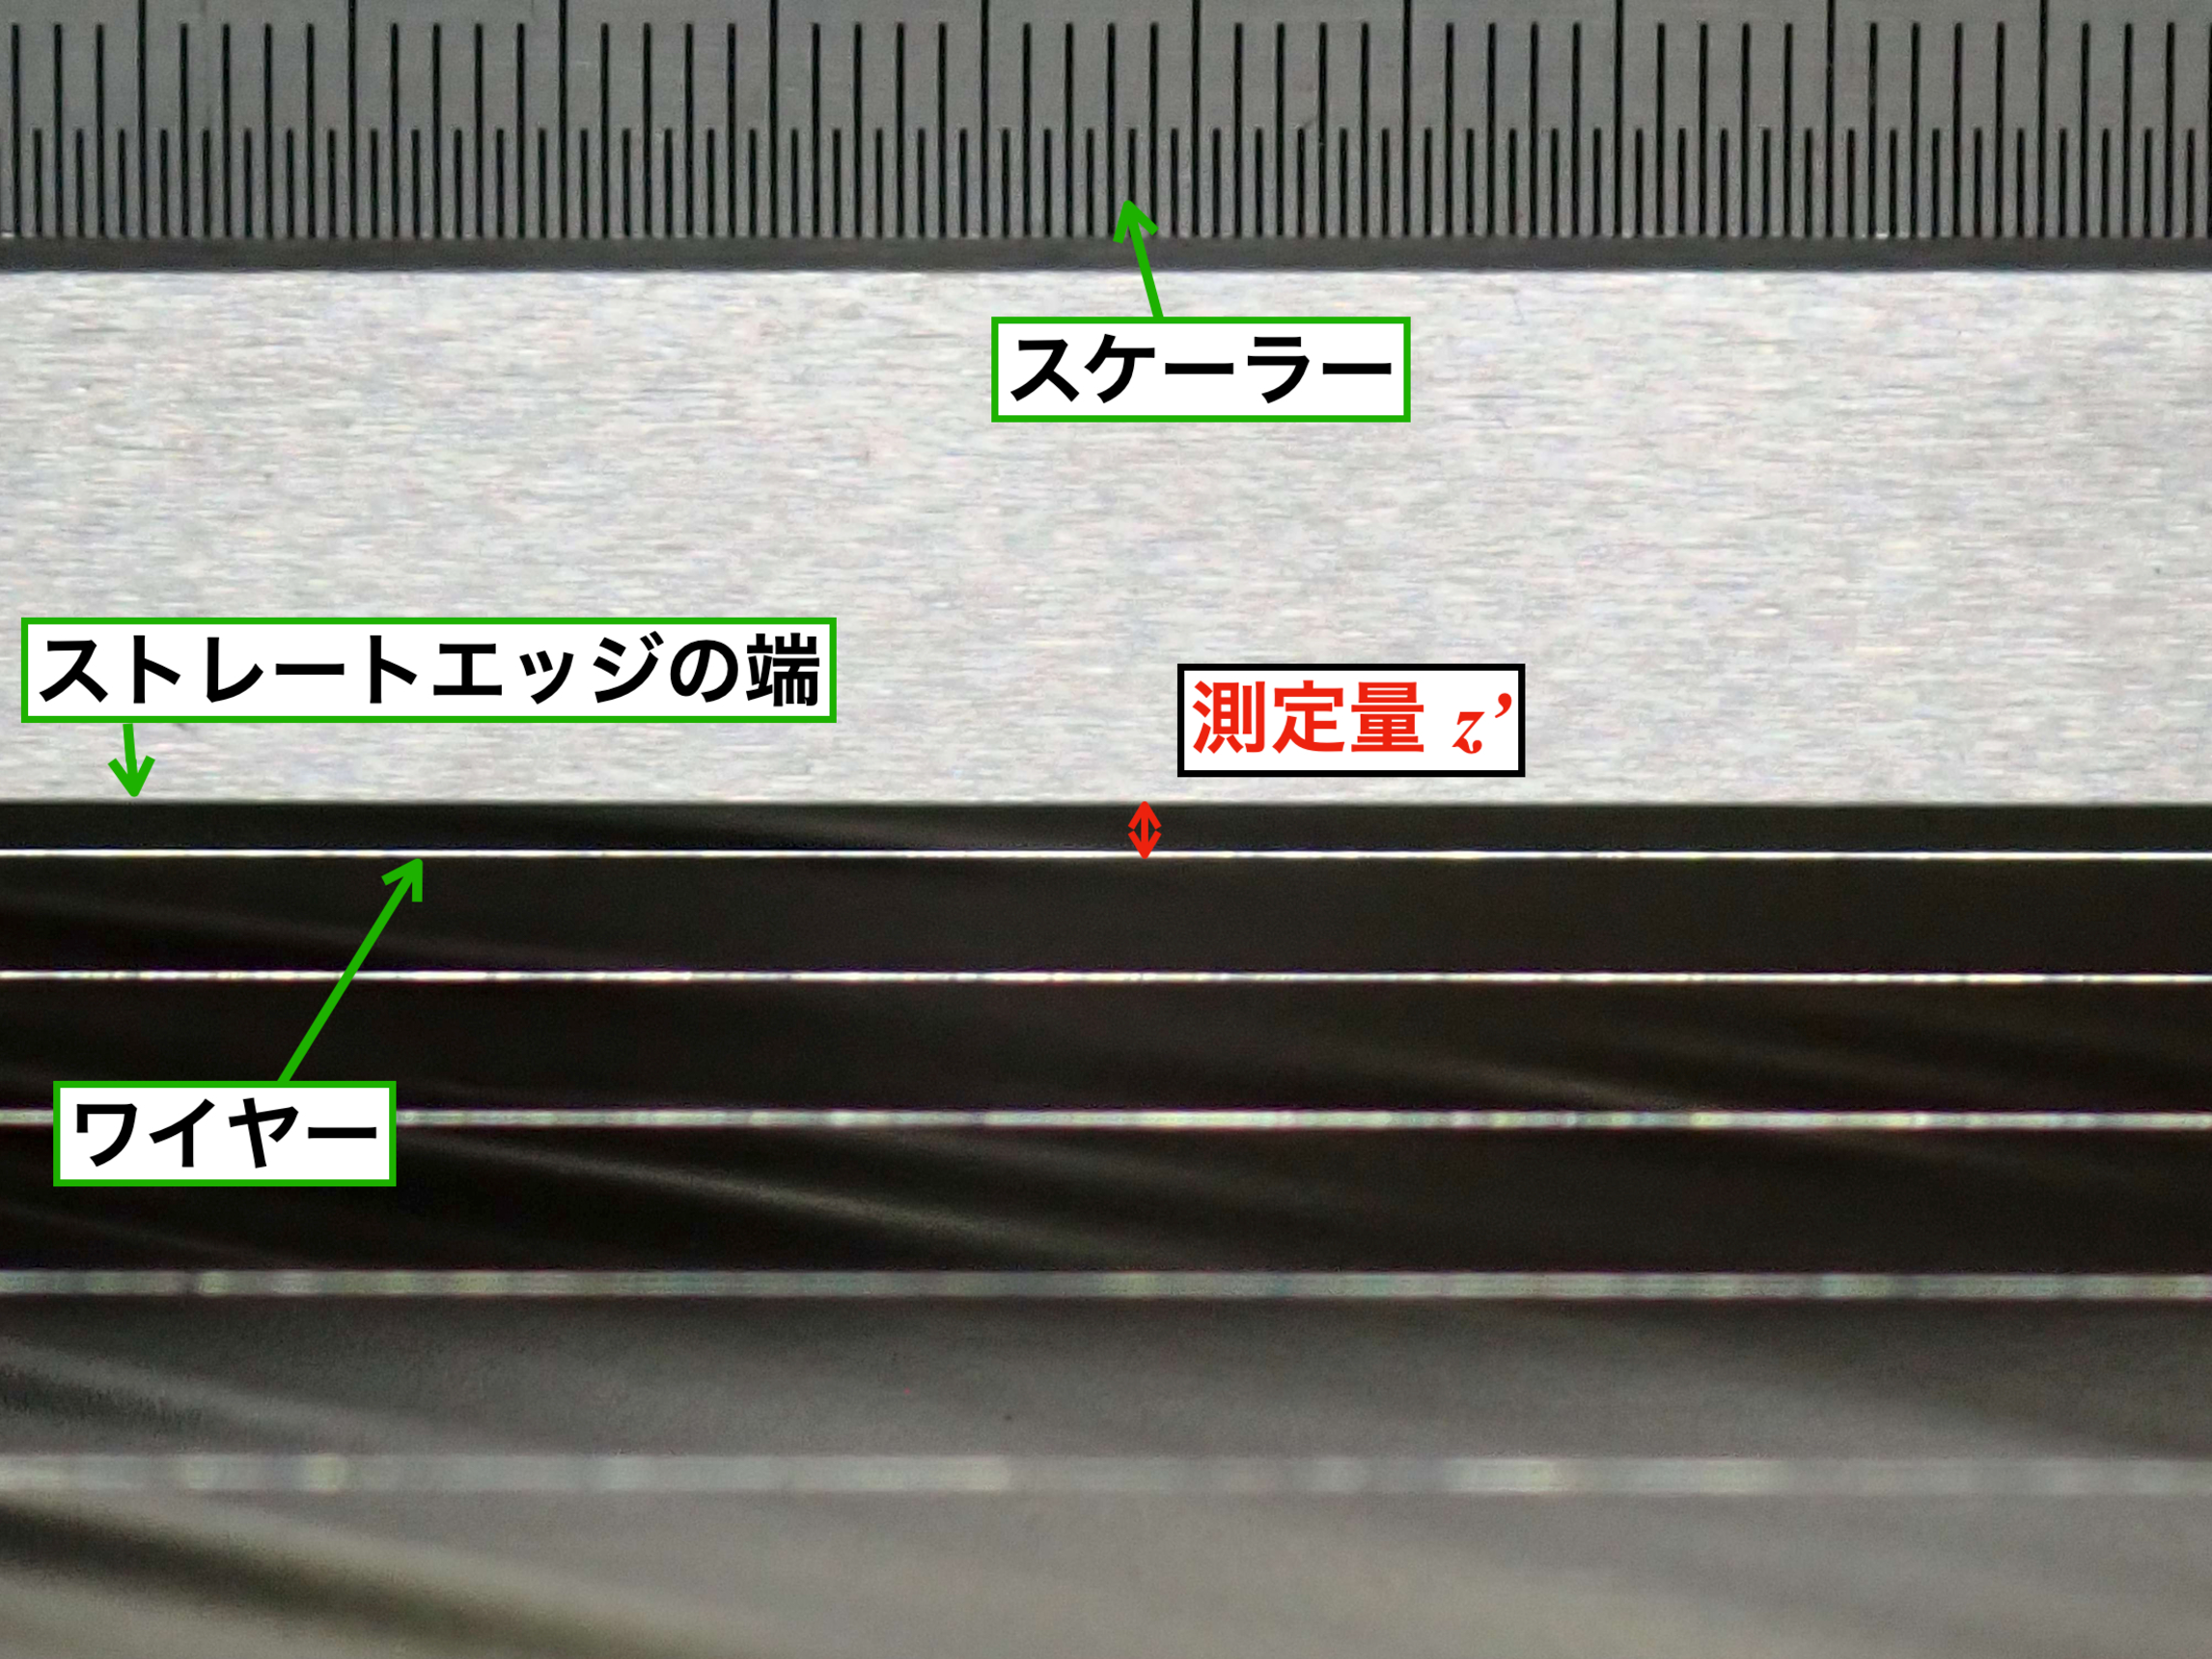
\includegraphics[width=0.8\textwidth]{wiregrid/wiresag_picture_old.pdf}
    \caption{ワイヤーのたわみ量評価の撮影された写真の例。}
    \label{fig:wiresag_picture_old}
\end{figure}
\subsection{系統誤差のまとめと本論文の位置付け}
表\ref{tab:systematic_errors_old}に、先行研究において調べられた系統誤差の結果をまとめる。
SOにおいて要求される絶対角度較正精度は $\delta\theta < 0.1\tcdegree$ であるが、
表\ref{tab:systematic_errors_old}中の評価値はこれを満たしていない。

特に問題となるのが重力参照計の精度である。要求精度を満たすため、
新たに Sherborne Sensors 社製の DSIC-2051-60 という重力参照計の導入を予定している。
この新しい重力参照計の精度の検証を、\ref{chap:tiltsensor}章にて行う。

次点で系統誤差を生んでいるワイヤーのたわみに関しては、写真の撮影箇所が両端と中心のみと少ないことや、
撮影箇所を人が決めていることに起因するバイアスが含まれている可能性がある。
さらに、観測サイトにおける品質管理の面を考えると、定期的に測定できるようなシステムの開発が望まれる。
こういった状況を受け、より正確にワイヤーのたわみ量を評価する手法と、その自動化手法を確立した。
\ref{chap:wiresag}章にてこの詳細を論ずる。

\begin{table}[H]
    \centering
    \caption{先行研究によって評価された系統誤差}
    \begin{tabular}{|c|c|}
        \hline
        系統誤差要因 & 評価値 \\
        \hline
        ワイヤー設置精度 & $< 0.02\tcdegree$ \\
        エンコーダ精度 & $<0.03\tcdegree$ \\
        エンコーダ零点 & $<0.04\tcdegree$ \\
        重力参照計 & $>0.1\tcdegree$ \\
        ワイヤーのたわみ & $<0.05\tcdegree$ \\
        \hline
        合計 & $>0.1\tcdegree$ \\
        \hline
    \end{tabular}
    \label{tab:systematic_errors_old}
\end{table}


\end{document}